%% \documentclass[handout,t]{beamer} % HANDOUT
\documentclass[handout,notes=show,t]{beamer} % NOTES
%% \documentclass[t]{beamer} % SLIDES

\usetheme{DSM}
\usepackage{beamer-tools-dsm}

%%
%% some useful macros: mathematical notation etc.
%%

%% abbreviations for logic symbols
\renewcommand{\implies}{\Rightarrow}
\newcommand{\equivalent}{\Leftrightarrow}

%% abbreviations for common number spaces
\newcommand{\setN}[1][]{\mathbb{N}_{#1}} % allows \setN and \setN[0]
\newcommand{\setZ}{\mathbb{Z}}
\newcommand{\setQ}{\mathbb{Q}}
\newcommand{\setR}{\mathbb{R}}

%% sets and (sub-)sets defined by condition
\newcommand{\set}[1]{\{#1\}}
\newcommand{\setdef}[2]{\set{#1\,|\,#2}}
\newcommand{\bigset}[1]{\bigl\{#1\bigr\}}
\newcommand{\bigsetdef}[2]{\bigset{#1\bigm|#2}}
\newcommand{\setscale}[1]{\left\{#1\right\}}
\newcommand{\setdefscale}[2]{\setscale{#1\left|\,#2\right.}}

%% absolute value and norm
\newcommand{\abs}[1]{\lvert #1\rvert}
\newcommand{\bigabs}[1]{\bigl\lvert #1\bigr\rvert}
\newcommand{\absscale}[1]{\left\lvert #1\right\rvert}
\newcommand{\norm}[2][]{\lVert #2\rVert_{#1}}
\newcommand{\bignorm}[2][]{\bigl\lVert #2\bigr\rVert_{#1}}
\newcommand{\normscale}[2][]{\left\lVert #2\right\rVert_{#1}}

%% complement set (with optional index)
\newcommand{\compl}[1][]{\mathcal{C}^{#1}}

%% power set: \powerset{\Sigma^*}
\newcommand{\powerset}[1]{\mathcal{P}(#1)}

%% uparrow: a \ua b = direct dominance in ordered tree
\newcommand{\ua}{\uparrow}

%% left-right arrow: this $\lra$ that
\newcommand{\lra}{\leftrightarrow}

%% expanded engineering notation: 4.2\x\e+5
\newcommand{\e}[2]{10^{\ifthenelse{\equal{#1}{+}}{}{#1}#2}}
\newcommand{\x}{\cdot}

%% arg max & min: \argmax_{x\in C}, \argmin_{x\in C}
\newcommand{\argmax}{\mathop{\text{arg~max}}}
\newcommand{\argmin}{\mathop{\text{arg~min}}}

%% infinitesimal elements: \dx, \dy = \dX{y}, \dz
\newcommand{\dX}[1]{\,\mathit{d{#1}}}
\newcommand{\dx}{\dX{x}}
\newcommand{\dy}{\dX{y}}
\newcommand{\dz}{\dX{z}}

%%% Local Variables: 
%%% mode: latex
%%% TeX-master: ""
%%% End: 
  % basic mathematical notation
%%
%% some macros for typesetting text
%%

%% \OPEN ... \CLOSE; \OPEN[np] ... \CLOSE[np]
%% bold large brackets for labelled bracketing notation
\newcommand<>{\OPEN}[1][]{\only#2{$\boldsymbol{\bigl[}\text{}_{\text{\raisebox{-2pt}{\textsc{#1}}}}$}}
\newcommand<>{\CLOSE}[1][]{\only#2{$\text{}_{\text{\raisebox{-2pt}{\textsc{#1}}}}\boldsymbol{\bigr]}$}}

%% \textgap ("_" representing missing letter)
\newcommand{\textgap}{\mbox{\hspace{.4pt}\texttt{\bfseries\secondary{\textunderscore}}\hspace{.4pt}}}

%% \textstar, \textast (math \star and \ast symbols in text mode, with some extra spacing)
\newcommand{\textstar}{$\mspace{.8mu}\star\mspace{.8mu}$}
\newcommand{\textast}{$\ast$}

%% $\p{\ctext{abc}}$ (cited text in mathematical equations, e.g. n-gram probabilities)
\newcommand{\ctext}[1]{\text{\textcite{#1}}}

%% $\p{\btext{abc}}$ (normal black text even in coloured math environment)
\newcommand{\btext}[1]{\text{\foreground{#1}}} 

%% text subscripts and superscripts (can be used in math and text mode)
\newcommand{\tsup}[1]{\ensuremath{^{\text{#1}}}}
\newcommand{\tsub}[1]{\ensuremath{_{\text{#1}}}}

%%% Local Variables: 
%%% mode: latex
%%% TeX-master: ""
%%% End: 
  % some useful macros for plain text
%%
%% some useful macros: statistical notation
%%

%% \p{X=k};  \pC{X=k}{Y=l};  \bigp{X_i = k};   \pscale{\frac{Z}{S^2}};
%% probability P(X=k) and conditional probability P(X=k|Y=l), also with larger or scaled parentheses
%% \p[\theta]{X=k};  \pC[\text{interpolated}]{X=k}{Y=l};  ...
%% with optional subscripts (for model probability, null probability, etc.)
\newcommand{\p}[2][]{\mathop{\mathrm{Pr}_{#1}}(#2)}
\newcommand{\pscale}[2][]{\mathop{\mathrm{Pr}_{#1}}\!\left(#2\right)}
\newcommand{\bigp}[2][]{\mathop{\mathrm{Pr}_{#1}}\bigl(#2\bigr)}
\newcommand{\pC}[3][]{\p[#1]{#2\,|\,#3}} 
\newcommand{\pCscale}[3][]{\pscale[#1]{#2\left|\,#3\right.\!}} 
\newcommand{\bigpC}[3][]{\bigp[#1]{#2\!\bigm|\!#3}} 

%% \Exp{X};  \Var{X};  \Exp[0]{X};  \Var[0]{X};  
%% \bigExp{X}; \bigVar{X}; \Expscale{X};  \Varscale{X};
%% expectation E[X] and variance V[X], expectation and variance under null hypothesis, 
%% and variants with largeer or scaled brackets
\newcommand{\Exp}[2][]{\mathrm{E}_{#1}[#2]}
\newcommand{\Var}[2][]{\mathop{\mathrm{Var}}_{#1}[#2]}
\newcommand{\bigExp}[2][]{\mathrm{E}_{#1}\!\bigl[#2\bigr]}
\newcommand{\bigVar}[2][]{\mathop{\mathrm{Var}}_{#1}\bigl[#2\bigr]}
\newcommand{\Expscale}[2][]{\mathrm{E}_{#1}\left[#2\right]}
\newcommand{\Varscale}[2][]{\mathop{\mathrm{Var}}_{#1}\left[#2\right]}

%% \pihat = \hat{\pi}
%% sampling estimate for population probability \pi (may need fine-tuning)
\newcommand{\pihat}{\hat{\pi}}

%% \Entropy{X}, \Entropy{p}, \KL{p}{q}, \MI{X}{Y}
%% \bigEntropy{}, \Entropyscale{}, \bigKL{}{}, \KLscale{}{}, \bigMI{}{}, \MIscale{}{}
%% entropy, KL distance, conditional entropy and mutual information (with scaled variants)
\newcommand{\Entropy}[1]{H[{#1}]}
\newcommand{\bigEntropy}[1]{H\bigl[{#1}\bigr]}
\newcommand{\Entropyscale}[1]{H\left[{#1}\right]}
\newcommand{\KL}[2]{D({#1}\|{#2})}
\newcommand{\bigKL}[2]{D\bigl({#1}\bigm\|{#2}\bigr)}
\newcommand{\KLscale}[2]{D\left({#1}\left\|{#2}\right.\right)}
\newcommand{\MI}[2]{I[{#1};{#2}]}
\newcommand{\bigMI}[2]{I\bigl[{#1};{#2}\bigr]}
\newcommand{\MIscale}[2]{I\left[{#1};{#2}\right]}

%% \corr (correlation) and \cov (covariance) as mathop's
\newcommand{\corr}{\mathop{\mathrm{corr}}}
\newcommand{\cov}{\mathop{\mathrm{cov}}
}
%%% Local Variables: 
%%% mode: latex
%%% TeX-master: ""
%%% End: 
  % notation for probability theory and statistics
%%
%% convenience macros for linear algebra (vectors and matrices)
%%

%% \Vector[i]{x} ... vector variable with optional _superscript_ index in parentheses
%% \Vector[']{x} ... special case: ' superscript not enclosed in parentheses
%% \vx, \vy, \vz ... abbreviations for common vector names
\newcommand{\Vector}[2][]{\mathbf{#2}\ifthenelse{\equal{#1}{}}{}{^{(#1)}}}
\newcommand{\vx}[1][]{\Vector[#1]{x}}
\newcommand{\vy}[1][]{\Vector[#1]{y}}
\newcommand{\vz}[1][]{\Vector[#1]{z}}
\newcommand{\vu}[1][]{\Vector[#1]{u}}
\newcommand{\vv}[1][]{\Vector[#1]{v}}
\newcommand{\vw}[1][]{\Vector[#1]{w}}
\newcommand{\va}[1][]{\Vector[#1]{a}} % vectors of coefficients
\newcommand{\vb}[1][]{\Vector[#1]{b}} % for basis
\newcommand{\vc}[1][]{\Vector[#1]{c}} % context vectors
\newcommand{\ve}[1][]{\Vector[#1]{e}} % for standard basis of R^n
\newcommand{\vm}[1][]{\Vector[#1]{m}} % row vectors of term-term matrix
\newcommand{\vn}[1][]{\Vector[#1]{n}} % normal vector
\newcommand{\vmu}[1][]{\Vector[#1]{\boldsymbol{\mu}}} % column vectors of term-term matrix
\newcommand{\vf}[1][]{\Vector[#1]{f}} % row vectors of term-context matrix
\newcommand{\vphi}[1][]{\Vector[#1]{\boldsymbol{\phi}}} % column vectors of term-context matrix
\newcommand{\vxi}[1][]{\Vector[#1]{\boldsymbol{\xi}}} % coordinate vector
\newcommand{\vnull}[1][]{\Vector[#1]{0}} % neutral element

%% \Span{\vb[1],\ldots,\vb[k]} ... span of set of vectors
%% \Rank{...} ... rank of set of vectors or matrix
%% \Det{...}, \det A ... determinant of a set of vectors / a matrix A
%% \Image{f}, \Kernel{f} ... image and kernel of a linear map
\newcommand{\Span}[1]{\mathop{\text{sp}}\left(#1\right)}
\newcommand{\Rank}[1]{\mathop{\text{rank}}\left(#1\right)}
\newcommand{\Det}[1]{\mathop{\text{Det}}\left(#1\right)}
%% \det is already defined in the standard library
\newcommand{\Image}[1]{\mathop{\text{Im}}\left(#1\right)}
\newcommand{\Kernel}[1]{\mathop{\text{Ker}}\left(#1\right)}

%% \dist[2]{\vx}{\vy} ... distance between two vectors (p-metric)
\newcommand{\dist}[3][]{d_{#1}\left(#2, #3\right)}
\newcommand{\bigdist}[3][]{d_{#1}\bigl(#2, #3\bigr)}

%% \sprod{\vu}{\vv} ... scalar product
\newcommand{\sprod}[2]{\left\langle #1, #2 \right\rangle}
\newcommand{\bigsprod}[2]{\bigl\langle #1, #2 \bigr\rangle}


%%% Local Variables: 
%%% mode: latex
%%% TeX-master: ""
%%% End: 
% convenience macros for vectors and matrices

%%%
%%% local configuration adjustments
%%%

%%% You can change pre-defined colours here, override built-in macros from the
%%% style definition and standard library, as well as define macros needed by
%%% all local documents.

%%% e.g. adjust counterpoint (dark green) for data projectors where greens are
%%% far too bright, as well as green component of light colour and pure green
%%% (of course, it's a better solution to adjust the gamma settings of your monitor)
%%
%% \definecolor{counterpoint}{rgb}{.1, .3, 0}
%% \definecolor{light}{rgb}{.45, .3, .55}
%% \definecolor{puregreen}{rgb}{0, .35, 0}

%% ----- extra packages we need to load

\usepackage{tikz}
\usepackage{alltt}              % code examples with nicely formatted comments
\usepackage{hieroglf}           % hieroglyph font for the archeology example
\usepackage{rotating}
\usepackage{multirow}

%% ----- general copyright message (authors may change between versions of the tutorial)
\newcommand{\dsmcopyright}{%
  Copyright \textcopyright\ 2009--2016 Evert, Lenci, Baroni \& Lapesa | 
  Licensed under CC-by-sa version 3.0}


%% ----- automatically show TOC reminder at beginning of each subsection
\AtBeginSubsection[]
{
  \begin{frame}
    \frametitle{Outline}
    \tableofcontents[current,currentsubsection]
  \end{frame}
}

%% ----- some useful macros for the SIGIL course

%% > plot(x,y)      \REM{this produces a scatterplot}
\newcommand{\REM}[2][\small]{\textsf{#1\color{primary}\# #2}}

\newenvironment{Rcode}[1][]{%
\setbeamercolor{block title}{fg=counterpoint,bg=counterpoint!15!white}%
\setbeamercolor{block body}{bg=counterpoint!5!white}\small%
\begin{block}{#1}\begin{alltt}\ungap[1]}{%
\ungap[1]\end{alltt}\end{block}}

%% nice colour for R output: \begin{Rout} .. \end{Rout}
%% -- ugly hack: I'm sure theres a better way to do this
\newenvironment{Rout}[1][\footnotesize]{%
  \begin{footnotesize}#1\color{secondary}\bfseries}{%
  \color{black}\mdseries\end{footnotesize}}

%% symbols for centroid vector and singular value matrix 
%% \newcommand{\vmu}[1][]{\boldsymbol{\mu}\ifthenelse{\equal{#1}{}}{}{^{(#1)}}}
\newcommand{\Msigma}{\boldsymbol{\Sigma}}

%% rotated column labels for table (to fit long text into narrow columns
\newcommand{\rotLabel}[2][60]{\begin{rotate}{#1}#2\end{rotate}}
 % local adjustments to configuration and macros

%%%%%%%%%%%%%%%%%%%%%%%%%%%%%%%%%%%%%%%%%%%%%%%%%%%%%%%%%%%%%%%%%%%%%%
%% Titlepage

\title[DSM Tutorial]{Distributional Semantic Models}
\subtitle{Tutorial at NAACL-HLT 2010, Los Angeles, CA\\
  --- part 2 ---}
\author[\textcopyright\ Evert/Baroni/Lenci]{%
  Stefan Evert\inst{1}\\
  {\small with contributions from Marco Baroni\inst{2} and Alessandro Lenci\inst{3}}}
\institute[CC-by-sa]{%
  \inst{1}University of Osnabrück, Germany
  \and
  \inst{2}University of Trento, Italy
  \and
  \inst{3}University of Pisa, Italy
}

\date[wordspace.collocations.de]{
  Los Angeles, 1 June 2010\\
  \light{\tiny \dsmcopyright}}

\begin{document}

\logo{
\includegraphics[width=2cm]{img/naacl_2010_icon}}
\frame{\titlepage}
\logo{}

%%%%%%%%%%%%%%%%%%%%%%%%%%%%%%%%%%%%%%%%%%%%%%%%%%%%%%%%%%%%%%%%%%%%%%

\section*{Outline}
\frame{ 
  \frametitle{Outline}
  \tableofcontents
}

%%%%%%%%%%%%%%%%%%%%%%%%%%%%%%%%%%%%%%%%%%%%%%%%%%%%%%%%%%%%%%%%%%%%%%

% -- \input slide sets from pages/ subdirectory
%%%%%%%%%%%%%%%%%%%%%%%%%%%%%%%%%%%%%%%%%%%%%%%%%%%%%%%%%%%%%%%%%%%%%%
\section{Some elements of matrix algebra}

%%%%%%%%%%%%%%%%%%%%%%%%%%%%%%%%%%%%%%%%%%%%%%%%%%%%%%%%%%%%%%%%%%%%%%
\subsection{Length \& distance}

% \begin{frame}
  \frametitle{Geometry and meaning}
  %% \framesubtitle{}

  \begin{itemize}
  \item So far: apply vector methods and matrix algebra to DSMs
  \item Geometric intuition: \primary{distance $\simeq$ semantic
      (dis)similarity}
    \begin{itemize}
    \item nearest neighbours
    \item clustering
    \item semantic maps
    \item representation for connectionist models
    \end{itemize}
  \itemhand We need a mathematical notion of distance!
  \end{itemize}
\end{frame}

%%% Local Variables: 
%%% mode: latex
%%% TeX-master: "../../workspace"
%%% End: 


\begin{frame}
  \frametitle{Measuring distance}
  %% \framesubtitle{}

  \begin{columns}[T]
    \begin{column}{60mm}
      \begin{itemize}
      \item \h{Distance} between vectors $\vu, \vv \in \setR^n$ \so
        (dis)\h{similarity}\\ of data points
        \begin{itemize}
        \item $\vu = (u_1, \ldots, u_n)$
        \item $\vv = (v_1, \ldots, v_n)$
        \end{itemize}
      \item \h{Euclidean} distance $\dist[2]{\vu}{\vv}$
      \item ``City block'' \h{Manhattan} distance $\dist[1]{\vu}{\vv}$
      \item Both are special cases of the \h{Minkowski} $p$-distance
        $\dist[p]{\vu}{\vv}$ (for $p\in [1, \infty]$)
      \end{itemize}
    \end{column}
    \begin{column}{40mm}
      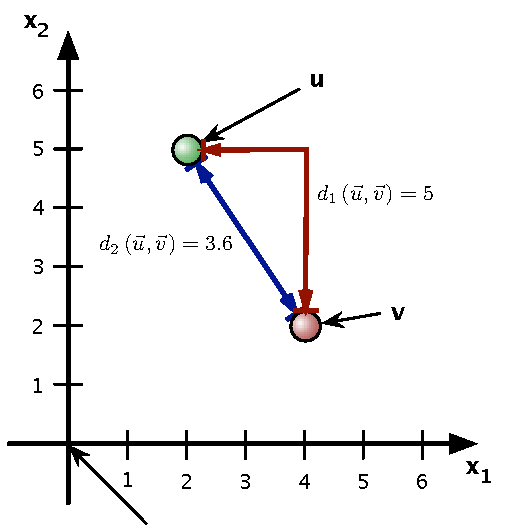
\includegraphics[width=40mm]{img/2_distance_examples}
    \end{column}
  \end{columns}
  \gap[.5]
    \[ \dist[p]{\vu}{\vv} \coloneq \bigl(
    \abs{u_1 - v_1}^p + \dots + \abs{u_n - v_n}^p
    \bigr)^{1/p} \] 
    %
    \[ \dist[\infty]{\vu}{\vv} = \max \bigset{\abs{u_1 - v_1}, \ldots, \abs{u_n - v_n}} \] 
\end{frame}

\begin{frame}
  \frametitle{Metric: a measure of distance}
  %% \framesubtitle{}

  \begin{itemize}
  \item A \h{metric} is a general measure of the distance $\dist{\vu}{\vv}$
    between points $\vu$ and $\vv$, which satisfies the following \h{axioms}:
    \begin{itemize}
      \item $\dist{\vu}{\vv} = \dist{\vv}{\vu}$
      \item $\dist{\vu}{\vv} > 0$ for $\vu \neq \vv$
      \item $\dist{\vu}{\vu} = 0$
      \item $\dist{\vu}{\vw} \leq \dist{\vu}{\vv} + \dist{\vv}{\vw}$
        (\h{triangle inequality})
    \end{itemize}
    \pause
  \item Metrics form a very broad class of distance measures, some of which do
    not fit in well with our geometric intuitions%
    \pause
  \item E.g., metric need not be \h{translation-invariant}
    \[ \dist{\vu+\vx}{\vv+\vx} \neq \dist{\vu}{\vv} \]
    \pause\ungap
  \item Another unintuitive example is the \hh{discrete metric}
    \[
    \dist{\vu}{\vv} =
    \begin{cases}
      0 & \vu = \vv \\
      1 & \vu \neq \vv
    \end{cases}
    \]
  \end{itemize}
\end{frame}

%%% Local Variables: 
%%% mode: latex
%%% TeX-master: "../../workspace"
%%% End: 


\begin{frame}
  \frametitle{Distance vs.\ norm}
  %% \framesubtitle{}

  \begin{columns}[T]
    \begin{column}{50mm}
      \begin{itemize}
      \item<1-> Intuitively, \h{distance} $\dist{\vu}{\vv}$ should correspond to
        \h{length} $\norm{\vu-\vv}$ of displacement vector $\vu - \vv$
        \begin{itemize}
        \item $\dist{\vu}{\vv}$ is a \h{metric}
        \item $\norm{\vu-\vv}$ is a \h{norm}
        \item $\norm{\vu} = \bigdist{\vu}{\vnull}$
        \end{itemize}
      \item<2-> Such a metric is always \h{translation-invariant}%
        \gap
      \item<3-> $\dist[p]{\vu}{\vv} = \norm[p]{\vv-\vu}$
      \end{itemize}
    \end{column}
    \begin{column}{50mm}
      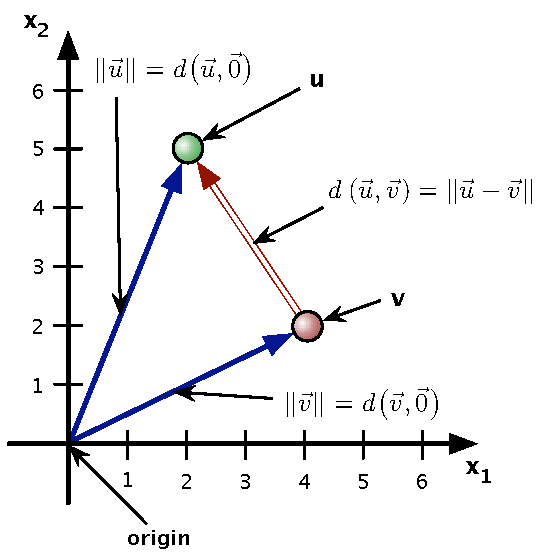
\includegraphics[width=50mm]{img/2_distance_norm}
    \end{column}
  \end{columns}

  \begin{itemize}
  \item<3-> \h{Minkowski $p$-norm} for $p\in [1,\infty]$:
    \[
    \norm[p]{\vu} \coloneq \bigl(\abs{u_1}^p + \dots + \abs{u_n}^p\bigr)^{1/p}
    \]
  \end{itemize}
\end{frame}

\begin{frame}
  \frametitle{Norm: a measure of length}
  %% \framesubtitle{}

  \begin{itemize}
  \item A general \h{norm} $\norm{\vu}$ for the length of a vector $\vu$ must
    satisfy the following \h{axioms}:
    \begin{itemize}
    \item $\norm{\vu} > 0$ for $\vu \neq \vnull$
    \item $\norm{\lambda\vu} = \abs{\lambda}\cdot \norm{\vu}$
      (\h{homogeneity}, not req'd for metric)
    \item $\norm{\vu + \vv} \leq \norm{\vu} + \norm{\vv}$
      (\h{triangle inequality})
    \end{itemize}
    \pause\gap
  \item every norm defines a translation-invariant metric
    \[ \dist{\vu}{\vv} \coloneq \norm{\vu - \vv} \]
  \end{itemize}
\end{frame}

\begin{frame}
  \frametitle{Norm: a measure of length}
  %% \framesubtitle{}

  \begin{columns}[T]
    \begin{column}{50mm}
      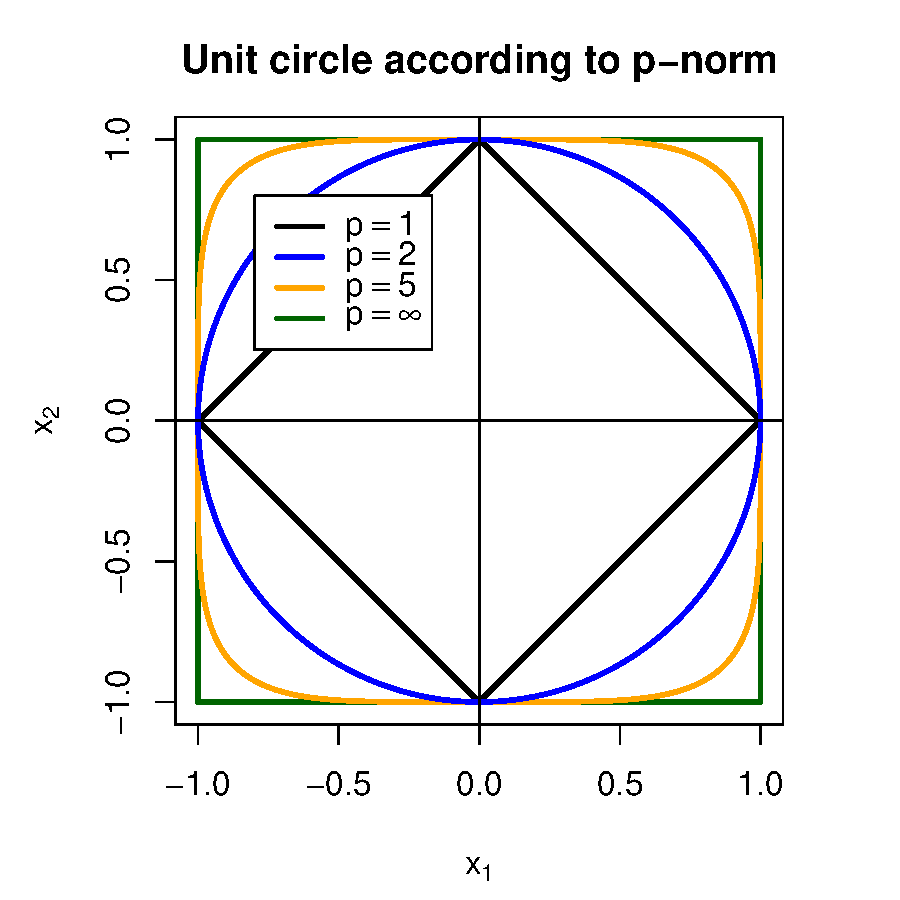
\includegraphics[width=50mm]{img/2_p_norms}
    \end{column}
    \begin{column}{50mm}
      \begin{itemize}
       \item Visualisation of norms in $\setR^2$ by plotting \h{unit
           circle} for each norm, i.e.\ points $\vu$ with $\norm{\vu}=1$
       \item Here: $p$-norms $\norm[p]{\cdot}$ for different values of $p$%
         \pause
       \item Triangle inequality $\iff$ unit circle is \h{convex}
       \item This shows that $p$-norms with $p < 1$ would violate the triangle
         inequality
      \end{itemize}
    \end{column}
  \end{columns}
  \pause%
  \begin{itemize}
  \item Consequence for DSM: $p \gg 2$ ``favours'' small differences in many
    coordinates, $p \ll 2$ differences in few coordinates
  \end{itemize}
\end{frame}

\begin{frame}
  \frametitle{Which metric should I use?}
  %% \framesubtitle{}

  \begin{itemize}
  \item Choice of metric or norm is one of the parameters of a DSM
    \pause
  \item Measures of \h{distance} between points:
    \begin{itemize}
    \item intuitive Euclidean norm $\norm[2]{\cdot}$
    \item ``city-block'' Manhattan distance $\norm[1]{\cdot}$
    \item maximum distance $\norm[\infty]{\cdot}$
    \item general Minkowski $p$-norm $\norm[p]{\cdot}$
    \item and many other formulae \ldots
    \end{itemize}
    \pause
  \item Measures of the \h{similarity} of arrows:
    \begin{itemize}
    \item ``cosine distance'' $\; \sim \ u_1 v_1 + \dots + u_n v_n$
    \item Dice coefficient (matching non-zero coordinates)
    \item and, of course, many other formulae \ldots
    \itemhand these measures determine \h{angles} between arrows
    \end{itemize}
    \pause
  \item Similarity and distance measures are equivalent!
    \begin{itemize}
    \item[\hand] I'm a fan of the Euclidean norm because of its intuitive
      geometric properties (angles, orthogonality, shortest path, \ldots)
    \end{itemize}
  \end{itemize}
\end{frame}

%%% Local Variables: 
%%% mode: latex
%%% TeX-master: "../../workspace"
%%% End: 


% \begin{frame}[fragile]
  \frametitle{Norms \& distance measures in R}
  %% \framesubtitle{}

\ungap
\begin{alltt}\small
\REM{We will use the cooccurrence matrix \textbf{M} from the last session}
> print(M)  \begin{Rout}
        eat get hear kill see use
  boat    0  59    4    0  39  23
  cat     6  52    4   26  58   4
  cup     1  98    2    0  14   6
  dog    33 115   42   17  83  10
  knife   3  51    0    0  20  84
  pig     9  12    2   27  17   3
\end{Rout}
\REM{Note: you can save selected variables with the \texttt{save()} command,}
\REM{and restore them in your next session (similar to saving R's workspace)}
> save(M, O, E, M.mds, file="dsm_lab.RData")

\REM{\texttt{load()} restores the variables under the same names!}
> load("dsm_lab.RData")
\end{alltt}
\end{frame}

\begin{frame}[fragile]
  \frametitle{Norms \& distance measures in R}
  %% \framesubtitle{}

\ungap
\begin{alltt}\small    
\REM{Define functions for general Minkowski norm and distance;}
\REM{parameter \emph{p} is optional and defaults to \emph{p} = 2}
> p.norm <- function (x, p=2) (sum(abs(x)^p))^(1/p)
> p.dist <- function (x, y, p=2) p.norm(x - y, p)

> round(apply(M, 1, p.norm, p=1), 2) \begin{Rout}
 boat   cat   cup   dog knife   pig 
  125   150   121   300   158    70 \end{Rout}
> round(apply(M, 1, p.norm, p=2), 2) \begin{Rout}
  boat    cat    cup    dog  knife    pig 
 74.48  82.53  99.20 152.83 100.33  35.44 \end{Rout}
> round(apply(M, 1, p.norm, p=4), 2) \begin{Rout}
  boat    cat    cup    dog  knife    pig 
 61.93  66.10  98.01 122.71  86.78  28.31 \end{Rout} 
> round(apply(M, 1, p.norm, p=99), 2) \begin{Rout}
 boat   cat   cup   dog knife   pig 
   59    58    98   115    84    27  \end{Rout}
\end{alltt}
\end{frame}

\begin{frame}[fragile]
  \frametitle{Norms \& distance measures in R}
  %% \framesubtitle{}

\ungap
\begin{alltt}\small    
\REM{Here's a nice trick to normalise the row vectors quickly}
> normalise <- function (M, p=2) M / apply(M, 1, p.norm, p=p)

\REM{\texttt{dist()} function also supports Minkowski \emph{p}-metric}
\REM{(must normalise rows in order to compare different metrics)}
> round(dist(normalise(M, p=1), method="minkowski", p=1), 2) \begin{Rout}
      boat  cat  cup  dog knife
cat   0.58                     
cup   0.69 0.97                
dog   0.55 0.45 0.89           
knife 0.73 1.01 1.01 1.00      
pig   1.03 0.64 1.29 0.71  1.28 \end{Rout}

\REM{Try different \emph{p}-norms: how do the distances change?}
> round(dist(normalise(M, p=2), method="minkowski", p=2), 2)
> round(dist(normalise(M, p=4), method="minkowski", p=4), 2)
> round(dist(normalise(M, p=99), method="minkowski", p=99), 2)
\end{alltt}
\end{frame}

\begin{frame}[c]
  \frametitle{Why it is important to normalise vectors}
  \framesubtitle{before computing a distance matrix}

  \begin{center}
    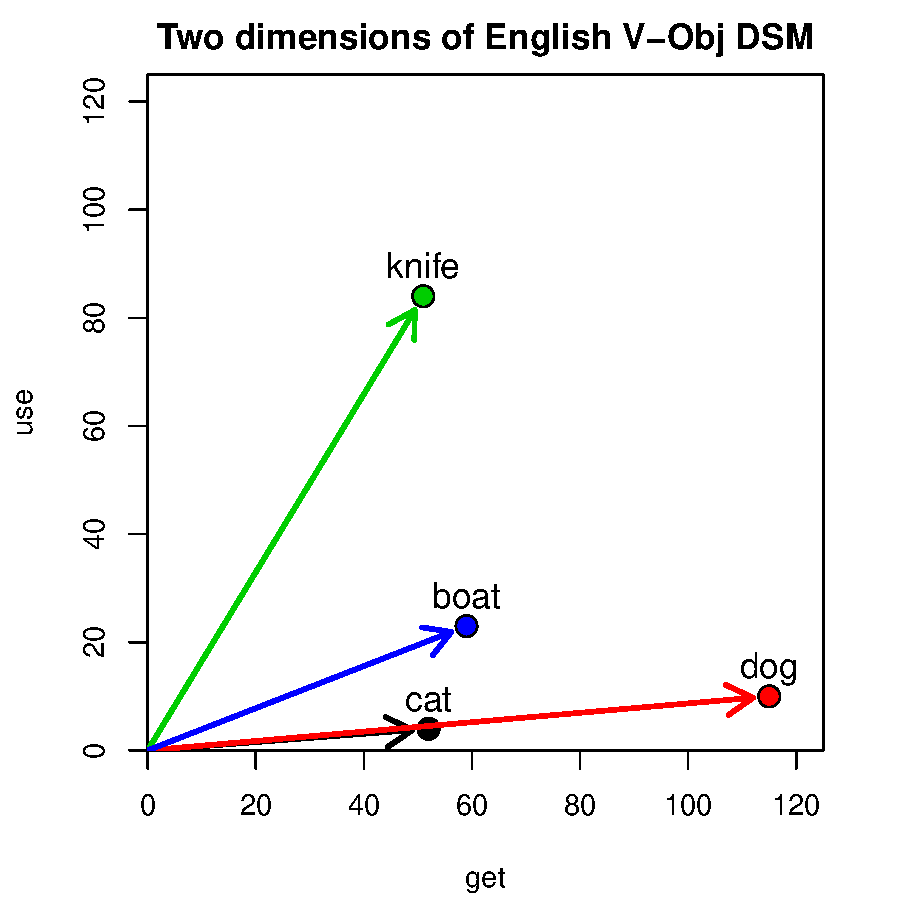
\includegraphics[width=7cm]{img/hieroglyph_2d_3}
  \end{center}
\end{frame}

%%% Local Variables: 
%%% mode: latex
%%% TeX-master: "../../workspace"
%%% End: 


%%%%%%%%%%%%%%%%%%%%%%%%%%%%%%%%%%%%%%%%%%%%%%%%%%%%%%%%%%%%%%%%%%%%%%
\subsection{Orientation}

\begin{frame}
  \frametitle{Euclidean norm \& inner product}
  %% \framesubtitle{}

  \begin{itemize}
  \item The Euclidean norm $\norm[2]{\vu} = \sqrt{\sprod{\vu}{\vu}}$ is
    special because it can be derived from the \h{inner product}:
    \[
    \sprod{\vu}{\vv} \coloneq \vx^T \vy = x_1 y_1 + \dots + x_n y_n
    \]
    where $\vu\equiv_E \vx$ and $\vv\equiv_E \vy$ are the standard coordinates
    of $\vu$ and $\vv$ (certain other coordinate systems also work)%
    \pause\gap
  \item The inner product is a \h{positive definite} and \h{symmetric}
    \h{bilinear form} with the following properties:
    \begin{itemize}
    \item $\sprod{\lambda \vu}{\vv} = \sprod{\vu}{\lambda \vv} = \lambda \sprod{\vu}{\vv}$
    \item $\sprod{\vu + \vu'}{\vv} = \sprod{\vu}{\vv} + \sprod{\vu'}{\vv}$
    \item $\sprod{\vu}{\vv + \vv'} = \sprod{\vu}{\vv} + \sprod{\vu}{\vv'}$
    \item $\sprod{\vu}{\vv} = \sprod{\vv}{\vu}$ (\h{symmetric})
    \item $\sprod{\vu}{\vu} = \norm{\vu}^2 > 0$ for $\vu \neq \vnull$ (\h{positive definite})
    \item also called \h{dot product} or \h{scalar product}
    \end{itemize}
  \end{itemize}
  \addnote{From now on, we will only consider Euclidean norms and metrics,
    omitting the subscript for brevity: $\norm{\cdot} = \norm[2]{\cdot}$.}%
\end{frame}

\begin{frame}
  \frametitle{Angles and orthogonality}
  %% \framesubtitle{}

  \begin{itemize}
  \item The Euclidean inner product has an important \h{geometric}
      interpretation \so angles and orthogonality%
    \pause
  \item \h{Cauchy-Schwarz inequality}:
    \[ \bigabs{\sprod{\vu}{\vv}} \leq \norm{\vu}\cdot \norm{\vv} \]
    \pause\ungap[1.5]
  \item \h{Angle} $\phi$ between vectors $\vu,\vv\in \setR^n$:
    \[ 
    \cos \phi \coloneq 
    \frac{\sprod{\vu}{\vv}}{\norm{\vu}\cdot \norm{\vv}}
    \]
    \ungap
    \begin{itemize}
    \item $\cos \phi$ is the ``cosine similarity'' measure
    \end{itemize}
    \pause
  \item $\vu$ and $\vv$ are \h{orthogonal} iff $\sprod{\vu}{\vv} = 0$
    \begin{itemize}
    \item the \h{shortest connection} between a point $\vu$ and a subspace $U$ is
      orthogonal to all vectors $\vv\in U$
    \end{itemize}
  \end{itemize}
\end{frame}

\begin{frame}[fragile]
  \frametitle{Cosine similarity in R}
  %% \framesubtitle{}

The \texttt{dist()} function does not calculate the cosine measure (because it
is a similarity rather than distance value), but:

\begin{small}
\[
\mathbf{M}\cdot \mathbf{M}^T = 
\begin{bmatrix}
  \cdots & \vu[1] & \cdots \\
  \cdots & \vu[2] & \cdots \\
  \\
  \\
  \cdots & \vu[n] & \cdots 
\end{bmatrix}
\cdot
\begin{bmatrix}
  \vdots & \vdots & & \vdots \\
  \vu[1] & \vu[2] & & \vu[n] \\
  \vdots & \vdots & & \vdots 
\end{bmatrix}
\]
\end{small}
\gap[.5]
\[
\text{\So}\quad
\bigl( \mathbf{M}\cdot \mathbf{M}^T \bigr)_{ij}
= \sprod{\vu[i]}{\vu[j]}
\]

\gap[0]
\begin{alltt}\small
\REM{Matrix of cosine similarities between rows of \textbf{M}:}
> M.norm <- normalise(M, p=2)  \REM{only works with Euclidean norm!}
> M.norm \%*\% t(M.norm)
\end{alltt}
\end{frame}

\begin{frame}[fragile]
  \frametitle{Euclidean distance or cosine similarity?}

  \begin{itemize}
  \item Which is better, Euclidean distance or cosine similarity?
  \item[]
  \item<2-> They are equivalent: if vectors are normalised ($\norm[2]{\vu} = 1$),
    both lead to the same neighbour ranking
  \end{itemize}

  \onslide<3->
  \begin{align*}
    \dist[2]{\vu}{\vv} 
    &= \sqrt{\norm[2]{\vu - \vv}}
    = \sqrt{\sprod{\vu - \vv}{\vu - \vv}}
    \\
    &= \sqrt{\sprod{\vu}{\vu} + \sprod{\vv}{\vv} - 2 \sprod{\vu}{\vv}}
    \\
    &= \sqrt{\norm[2]{\vu} + \norm[2]{\vv} - 2 \sprod{\vu}{\vv}}
    \\
    &= \sqrt{2 - 2 \cos \phi}
  \end{align*}
\end{frame}

\begin{frame}[c]
  \frametitle{Euclidean distance and cosine similarity}

  \begin{center}
    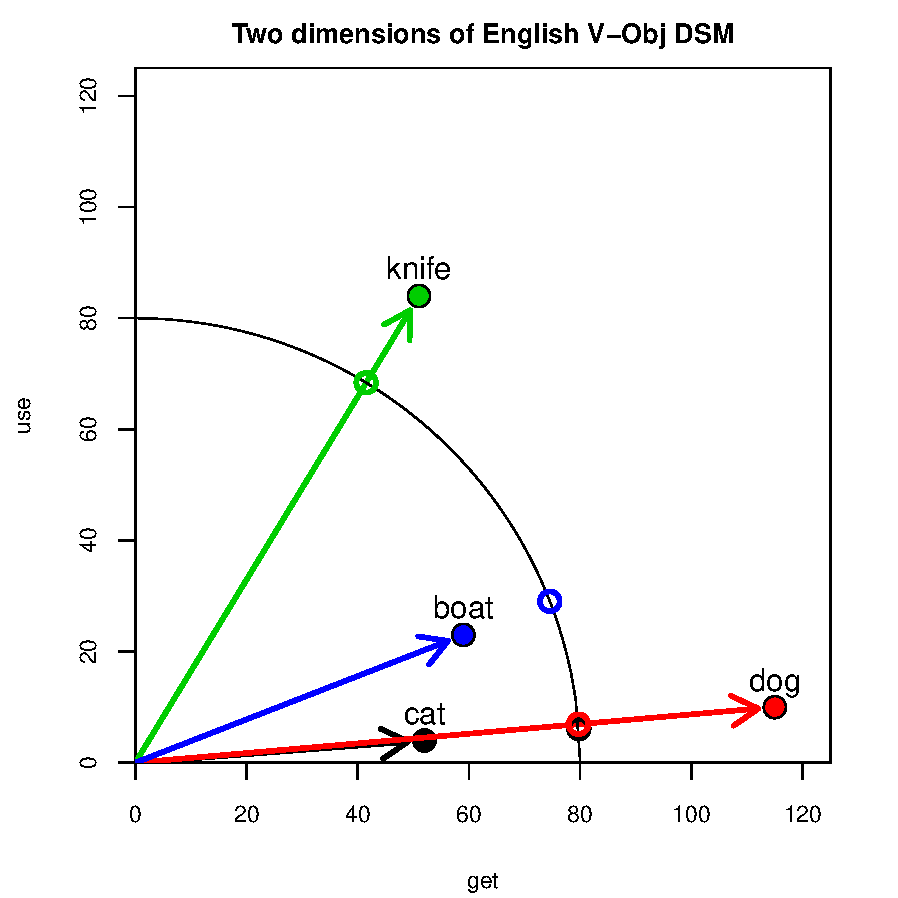
\includegraphics[width=7cm]{img/hieroglyph_2d_4}
  \end{center}
\end{frame}


\begin{frame}
  \frametitle{Cartesian coordinates}
  %% \framesubtitle{}

  \begin{itemize}
  \item A set of vectors $\vb[1], \ldots, \vb[n]$ is called \h{orthonormal} if
    the vectors are pairwise orthogonal and of unit length:
    \begin{itemize}
    \item $\bigsprod{\vb[j]}{\vb[k]} = 0$ for $j\neq k$
    \item $\bigsprod{\vb[k]}{\vb[k]} = \bignorm{\vb[k]}^2 = 1$
    \end{itemize}
  \item An orthonormal basis and the corresponding coordinates are called
    \h{Cartesian}%
    \pause
  \item Cartesian coordinates are particularly intuitive, and the inner
    product has the same form wrt.\ every Cartesian basis $B$: for $\vu\equiv_B
    \vx'$ and $\vv\equiv_B \vy'$, we have
    \[ \sprod{\vu}{\vv} = (\vx')^T \vy' = x'_1 y'_1 + \dots + x'_n y'_n \]
  \item NB: the column vectors of the matrix $\mathbf{B}$ are orthonormal%
    \begin{itemize}
    \item recall that the columns of $\mathbf{B}$ specify the standard
      coordinates of the vectors $\vb[1], \ldots, \vb[n]$
    \end{itemize}
  \end{itemize}
\end{frame}

\begin{frame}
  \frametitle{Orthogonal projection} 
  %% \framesubtitle{}
  
  \begin{itemize}
  \item Cartesian coordinates $\vu \equiv_B \vx$ can easily be computed:
    \begin{align*}
      \sprod{\vu}{\vb[k]} &= \sprod{\sum_{j=1}^n x_j \vb[j]}{\vb[k]} \\
      &= \sum_{j=1}^n x_j \underbrace{\sprod{\vb[j]}{\vb[k]}}_{= \delta_{jk}} 
      = x_k
    \end{align*}
    \begin{itemize}\ungap
    \item Kronecker delta: $\delta_{jk} = 1$ for $j=k$ and $0$ for $j\neq k$
    \end{itemize}
    \pause\gap
  \item \h{Orthogonal projection} $P_V:\setR^n\to V$ to subspace $V
    \coloneq \Span{\vb[1], \ldots, \vb[k]}$ (for $k < n$) is given by
    \[
    P_V \vu \coloneq \sum_{j=1}^k \vb[j] \sprod{\vu}{\vb[j]}
    \]
  \end{itemize}
\end{frame}

%%% Local Variables: 
%%% mode: latex
%%% TeX-master: "../../workspace"
%%% End: 


\begin{frame}
  \frametitle{Hyperplanes \& normal vectors}
  \framesubtitle{A hyperplane is the decision boundary of a linear classifier!}

  \begin{itemize}
  \item A hyperplane $U\subseteq \setR^n$ through the origin $\vnull$ can be
    characterized by the equation
    \[ U = \bigsetdef{\vu\in\setR^n}{\sprod{\vu}{\vn} = 0} \]
    for a suitable $\vn\in\setR^n$ with $\norm{\vn} = 1$
  \item $\vn$ is called the \h{normal vector} of $U$
  \item<2-> The orthogonal projection $P_U$ into $U$ is given by
    \[ P_U \vv \coloneq \vv - \vn \sprod{\vv}{\vn} \]
  \item<3-> An arbitrary hyperplane $\Gamma\subseteq \setR^n$ can analogously
    be characterized by
    \[ \Gamma = \bigsetdef{\vu\in\setR^n}{\sprod{\vu}{\vn} = a} \]
    where $a\in \setR$ is the (signed) \h{distance} of $\Gamma$ from $\vnull$
  \end{itemize}
\end{frame}

%%% Local Variables: 
%%% mode: latex
%%% TeX-master: "../../workspace"
%%% End: 


\begin{frame}
  \frametitle{Orthogonal matrices} 
  %% \framesubtitle{}

  \begin{itemize}
  \item A matrix $\mathbf{A}$ whose column vectors are orthonormal is called\\
    an \h{orthogonal} matrix
  \item $\mathbf{A}^T$ is orthogonal iff $\mathbf{A}$ is orthogonal%
    \pause\gap
  \item The \h{inverse} of an orthogonal matrix is simply its transpose:
    \[
    \mathbf{A}^{-1} = \mathbf{A}^T \quad \text{if $\mathbf{A}$ is orthogonal}
    \]
    \ungap[1]
    \begin{itemize}
    \item it is easy to show $\mathbf{A}^T \mathbf{A} = \mathbf{I}$ by matrix
      multiplication,\\ since the columns of $\mathbf{A}$ are orthonormal
    \item since $\mathbf{A}^T$ is also orthogonal, it follows that $\mathbf{A}
      \mathbf{A}^T = (\mathbf{A}^T)^T \mathbf{A}^T = \mathbf{I}$
    \item side remark: the transposition operator $\cdot^T$ is called\\
      an \hh{involution} because $(\mathbf{A}^T)^T = \mathbf{A}$
    \end{itemize}
  \end{itemize}
\end{frame}

\begin{frame}
  \frametitle{Isometric maps} 
  %% \framesubtitle{}

  \begin{itemize}
  \item An endomorphism $f: \setR^n \to \setR^n$ is called an \h{isometry} iff
    $\sprod{f(\vu)}{f(\vv)} = \sprod{\vu}{\vv}$ for all $\vu,\vv\in \setR^n$%
  \item Geometric interpretation: isometries preserve angles and distances
    (which are defined in terms of $\sprod{\cdot}{\cdot}$)%
    \pause
  \item $f$ is an isometry iff its matrix $\mathbf{A}$ is orthogonal%
    \pause
  \item Coordinate transformations between Cartesian systems are isometric
    (because $\mathbf{B}$ and $\mathbf{B}^{-1} = \mathbf{B}^T$ are orthogonal)%
    \pause
  \item Every isometric endomorphism of $\setR^n$ can be written as a
    combination of \hh{planar rotations} and \hh{axial reflections} in a
    suitable Cartesian coordinate system
      \[\footnotesize
      R_{\phi}^{(1,3)} = 
      \begin{bmatrix}
        \cos \phi & 0 & -\sin \phi \\
        0         & 1 &  0         \\
        \sin \phi & 0 &  \cos \phi 
      \end{bmatrix}, 
      \quad
      Q^{(2)} = 
      \begin{bmatrix}
        1 &  0 & 0 \\
        0 & -1 & 0 \\
        0 &  0 & 1
      \end{bmatrix}
      \]
  \end{itemize}
\end{frame}

\begin{frame}
  \frametitle{Summary: orthogonal matrices}
  %% \framesubtitle{}

  \begin{itemize}
  \item The column vectors of an orthogonal $n\times n$ matrix $\mathbf{B}$
    form a Cartesian basis $\vb[1],\ldots,\vb[n]$ of $\setR^n$%
    \pause
  \item $\mathbf{B}^{-1} = \mathbf{B}^T$, i.e.\ we have $\mathbf{B}^T
    \mathbf{B} = \mathbf{B} \mathbf{B}^T = \mathbf{I}$%
    \pause
  \item The coordinate transformation $\mathbf{B}^T$ into $B$-coordinates is an
    isometry, i.e.\ all distances and angles are preserved%
    \pause
  \item The first $k < n$ columns of $\mathbf{B}$ form a Cartesian basis of a
    subspace $V = \Span{\vb[1],\ldots,\vb[k]}$ of $\setR^n$%
    \pause
  \item The corresponding rectangular matrix $\mathbf{\hat{B}} =
    \bigl[\vb[1],\ldots,\vb[k]\bigr]$ performs an orthogonal projection into
    $V$:
    \begin{align*}
      P_V \vu  &\:\equiv_{B}\: \mathbf{\hat{B}}^T \vx 
      \qquad \text{(for } \vu \equiv_E \vx \text{)}\\
      &\:\equiv_{E}\: \mathbf{\hat{B}} \mathbf{\hat{B}}^T \vx 
    \end{align*}
  \item[\So] These properties will become important later today!
\end{itemize}
\end{frame}



%%% Local Variables: 
%%% mode: latex
%%% TeX-master: "../../workspace"
%%% End: 


% \begin{frame}
  \frametitle{General inner products} 
  %% \framesubtitle{}
  
  \begin{itemize}
  \item Can we also introduce geometric notions such as angles and orthogonality
    for other metrics, e.g.\ the Manhattan distance?
    \begin{itemize}
    \item[\hand] norm must be derived from appropriate inner product
    \end{itemize}
    \pause\gap
  \item General \h{inner products} are defined by
    \[ 
    \sprod{\vu}{\vv}_B \coloneq (\vx')^T \vy' = x'_1 y'_1 + \dots + x'_ y y'_n 
    \] 
    wrt.\ non-Cartesian basis $B$ ($\vu \equiv_B \vx'$, $\vv \equiv_B \vy'$)%
    \pause\gap
  \item $\sprod{\cdot}{\cdot}_B$ can be expressed in standard coordinates
    $\vu\equiv_E \vx$, $\vv \equiv_E \vy$ using the transformation matrix
    $\mathbf{B}$:
    \begin{align*}
      \sprod{\vu}{\vv}_B &= (\vx')^T \vy' 
      = \bigl( \mathbf{B}^{-1} \vx \bigr)^T \bigl( \mathbf{B}^{-1} \vy \bigr) \\
      &= \vx^T (\mathbf{B}^{-1})^T \mathbf{B}^{-1} \vy \eqcolon \vx^T \mathbf{C} \vy
    \end{align*}
  \end{itemize}
\end{frame}

\begin{frame}
  \frametitle{General inner products} 
  %% \framesubtitle{}
  
  \begin{itemize}
  \item The coefficient matrix $\mathbf{C} \coloneq (\mathbf{B}^{-1})^T
    \mathbf{B}^{-1}$ of the general inner product is \h{symmetric}
    \[
    \mathbf{C}^T = (\mathbf{B}^{-1})^T ((\mathbf{B}^{-1})^T)^T =
    (\mathbf{B}^{-1})^T \mathbf{B}^{-1} = \mathbf{C}
    \]
    \pause
    and \h{positive definite}
    \[
    \vx^T \mathbf{C} \vx 
    = \bigl( \mathbf{B}^{-1} \vx \bigr)^T \bigl( \mathbf{B}^{-1} \vx \bigr)
    = (\vx')^T \vx' \geq 0
    \]
    \pause
  \item It is (relatively) easy to show that every positive definite and
    symmetric bilinear form can be written in this way.
    \begin{itemize}
    \item[\hand] i.e.\ every norm that is derived from an inner product can be
      expressed in terms of a coefficient matrix $\mathbf{C}$ or basis $B$
    \end{itemize}
  \end{itemize}
\end{frame}

\begin{frame}
  \frametitle{General inner products} 
  %% \framesubtitle{}
  
  \begin{columns}[T]
    \begin{column}{50mm}
      An example:
      \begin{itemize}\gap
      \item $\vb[1] = (3,2)$, $\vb[2] = (1,2)$
      \item \(
        \mathbf{B} = \begin{bmatrix}
          3 & 1 \\ 2 & 2
        \end{bmatrix} \)
      \item \(
        \mathbf{B}^{-1} = \begin{bmatrix}
          \frac12 & -\frac14 \\ -\frac12 & \frac34
        \end{bmatrix} \)
      \item \(
        \mathbf{C} = \begin{bmatrix}
          .5 & -.5 \\ -.5 & .625
        \end{bmatrix} \)
      \item Graph shows \hh{unit circle} of the inner product $\mathbf{C}$, i.e.\
        points $\vx$ with \[ \vx^T \mathbf{C} \vx = 1 \]
      \end{itemize}
    \end{column}
    \begin{column}{50mm}
      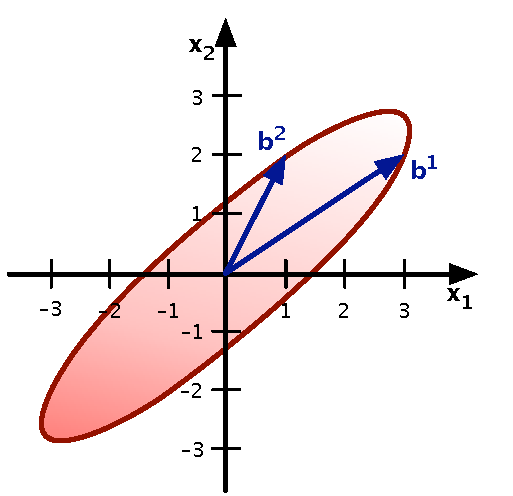
\includegraphics[width=50mm]{img/2_inner_product_1}
    \end{column}
  \end{columns}
\end{frame}

\begin{frame}
  \frametitle{General inner products} 
  %% \framesubtitle{}
  
  \begin{columns}[T]
    \begin{column}{50mm}
      \begin{itemize}\gap
      \item $\mathbf{C}$ is a symmetric matrix
      \item There is always an orthonormal basis such that $\mathbf{C}$ has
        diagonal form
      \item ``Standard'' dot product with additional scaling factors
        (wrt.\ this orthonormal basis)
      \item Intuition: unit circle is a squashed and rotated disk
      \end{itemize}
    \end{column}
    \begin{column}{50mm}
      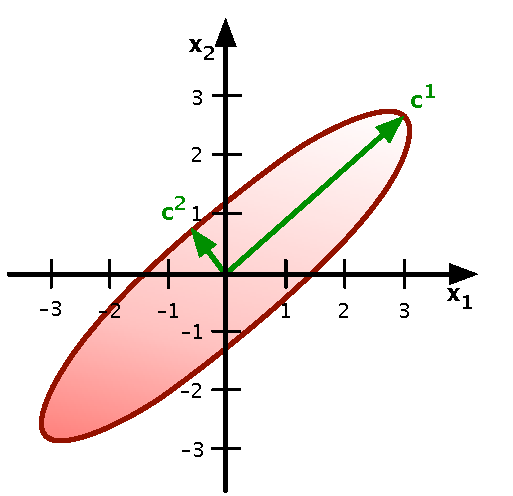
\includegraphics[width=50mm]{img/2_inner_product_2}
    \end{column}
  \end{columns}
  \begin{itemize}
  \item<2->[\So] Every ``geometric'' norm is equivalent to the Euclidean norm
    except for a rotation and rescaling of the axes
  \end{itemize}
\end{frame}

%%% Local Variables: 
%%% mode: latex
%%% TeX-master: "../../workspace"
%%% End: 


%%%%%%%%%%%%%%%%%%%%%%%%%%%%%%%%%%%%%%%%%%%%%%%%%%%%%%%%%%%%%%%%%%%%%%
\subsection{PCA}

% \begin{frame}
%   \frametitle{Motivating latent dimensions: example data}
%   %% \framesubtitle{}

%   \begin{columns}
%     \begin{column}{6.5cm}
%       \begin{itemize}
%       \item Example: term-term matrix
%       \item V-Obj cooc's extracted from BNC
%         \begin{itemize}
%         \item targets = noun lemmas\\
%         \item features = verb lemmas
%         \end{itemize}
%       \item feature scaling: association scores (modified $\log$ Dice
%         coefficient)
%       \item $k=111$ nouns with $f \geq 20$\\
%         (must have non-zero row vectors)
%       \item $n=2$ dimensions: \emph{buy} and \emph{sell}
%       \end{itemize}
%     \end{column}
%     \begin{column}{4cm}
%       \begin{center}\footnotesize
%         \begin{tabular}{l|rr}
%           noun & \emph{buy} & \emph{sell} \\
%           \hline
%           \emph{bond}      &  0.28 &  0.77\\
%           \emph{cigarette} & -0.52 &  0.44\\
%           \emph{dress}     &  0.51 & -1.30\\
%           \emph{freehold}  & -0.01 & -0.08\\
%           \emph{land}      &  1.13 &  1.54\\
%           \emph{number}    & -1.05 & -1.02\\
%           \emph{per}       & -0.35 & -0.16\\
%           \emph{pub}       & -0.08 & -1.30\\
%           \emph{share}     &  1.92 &  1.99\\
%           \emph{system}    & -1.63 & -0.70
%         \end{tabular}
%       \end{center}
%     \end{column}
%   \end{columns}
% \end{frame}

% \begin{frame}[c]
%   \frametitle{Motivating latent dimensions \& subspace projection}
%   %% \framesubtitle{}
%   \begin{center}
%     \ungap[1]
%     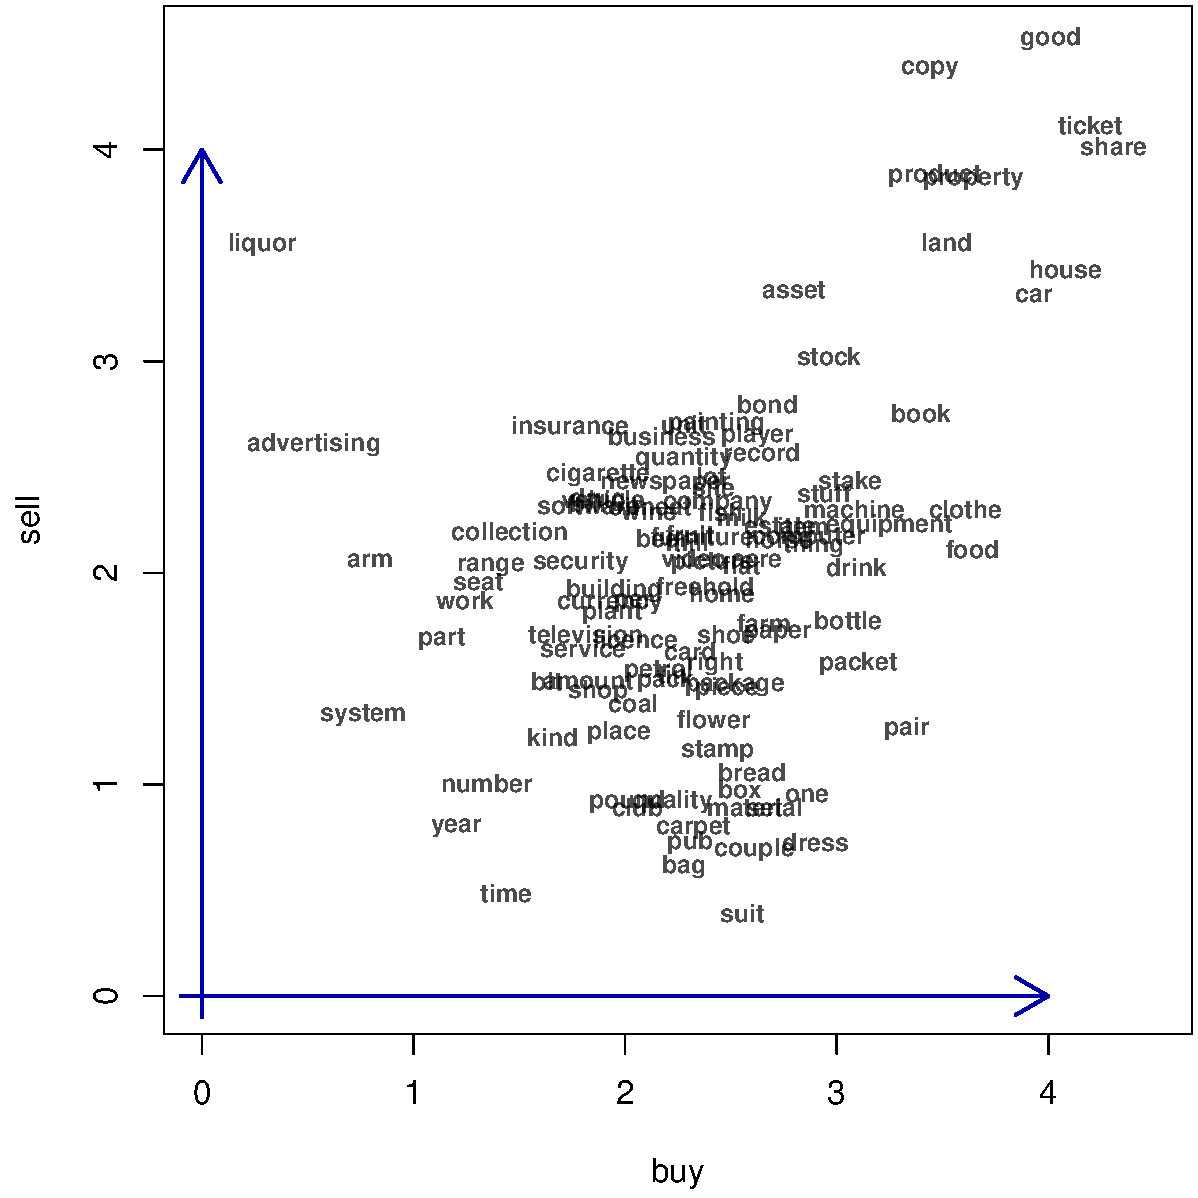
\includegraphics[width=8cm]{img/3_buy_sell_labels_only}
%   \end{center}
% \end{frame}

\begin{frame}
  \frametitle{Motivating latent dimensions \& subspace projection}
  %% \framesubtitle{}

  \begin{itemize}
  \item The \h{latent property} of being a commodity is ``expressed''
    through associations with several verbs: \emph{sell}, \emph{buy},
    \emph{acquire}, \ldots
  \item Consequence: these DSM dimensions will be \h{correlated}
  \item[]
  \item Identify \h{latent dimension} by looking for strong correlations\\
    (or weaker correlations between large sets of features)%
  \item Projection into subspace $V$ of $k < n$ latent dimensions\\
    as a ``\h{noise reduction}'' technique \so \hh{LSA}
  \item Assumptions of this approach:
    \begin{itemize}
    \item ``latent'' distances in $V$ are semantically meaningful
    \item other ``residual'' dimensions represent chance co-occurrence
      patterns, often particular to the corpus underlying the DSM
    \end{itemize}
  \end{itemize}
\end{frame}

\begin{frame}[c]
  \frametitle{The latent ``commodity'' dimension}
  %% \framesubtitle{}
  \begin{center}
    \ungap[1]
    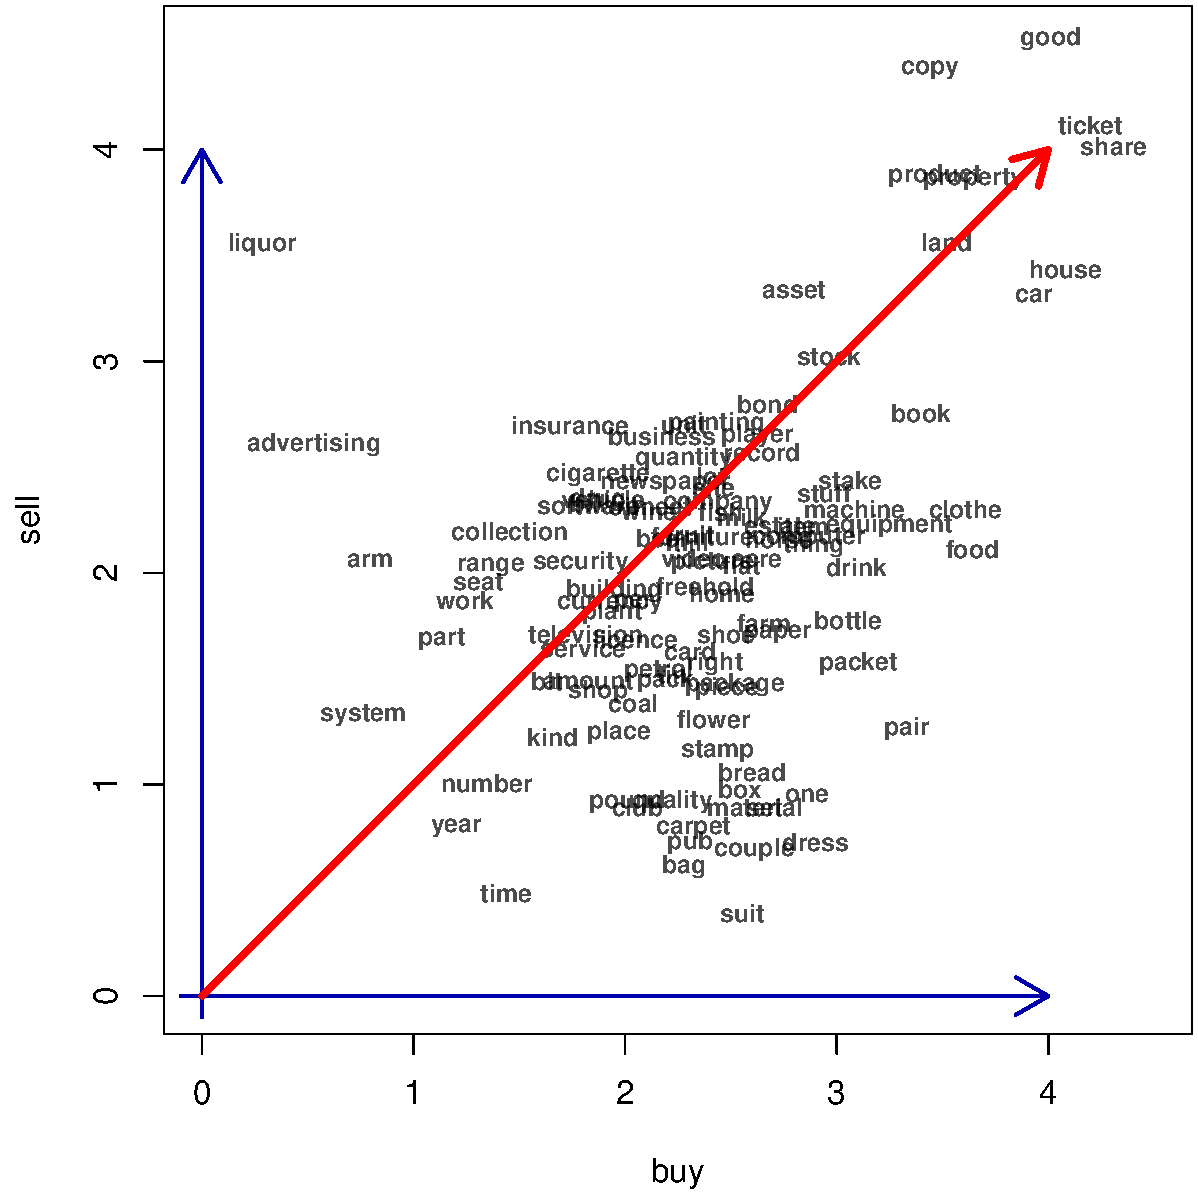
\includegraphics[width=8cm]{img/3_buy_sell_labels_latent}
  \end{center}
\end{frame}

%%% Local Variables: 
%%% mode: latex
%%% TeX-master: "../../workspace"
%%% End: 


\begin{frame}
  \frametitle{The variance of a data set}
  %% \framesubtitle{}

  \begin{itemize}
  \item Rationale: find the dimensions that give the best (statistical)
    explanation for the \h{variance} (or ``spread'') of the data
  \item Definition of the variance of a set of vectors
    \begin{itemize}
    \item[\hand] you remember the equations for one-dimensional data, right?
    \end{itemize}
    \ungap\pause
    \begin{align*}
      \sigma^2 &= \frac{1}{k-1} \sum_{i=1}^k \norm{\vx[i] - \vmu}^2 \\
      \vmu &= \frac{1}{k} \sum_{i=1}^k \vx[i]
    \end{align*}
  \item Easier to calculate if we \h{center} the data so that $\vmu = \vnull$
  \end{itemize}
\end{frame}

\begin{frame}[c]
  \frametitle{Centering the data set}
  %% \framesubtitle{}

  \begin{columns}[c]
    \begin{column}{40mm}
      \begin{itemize}
      \item \h<beamer:1| handout:1>{Uncentered\\ data set}%
        \gap
      \item \h<beamer:2| handout:2>{Centered\\ data set}%
        \gap
      \item \h<beamer:3| handout:3>{Variance of\\ centered data}%
        \gap
      \end{itemize}
      \visible<beamer:3| handout:3>{%
        \[
        \sigma^2 = \tfrac{1}{k-1} \sum_{i=1}^k \norm{\vx[i]}^2
        \]
      }
    \end{column}
    \begin{column}{60mm}
      \only<beamer:1| handout:1>{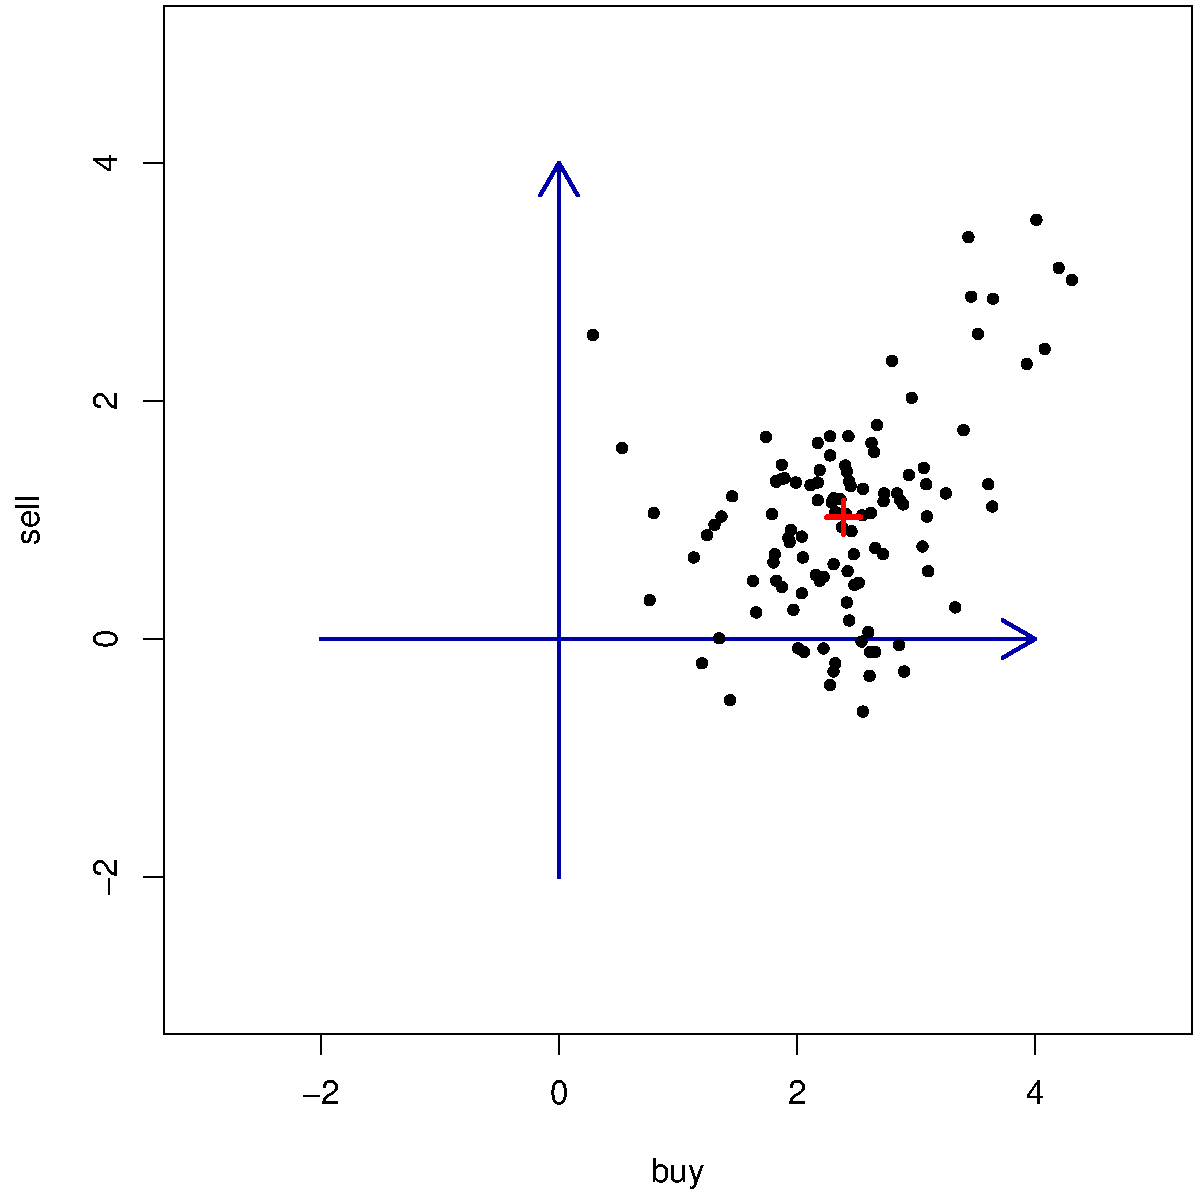
\includegraphics[width=6cm]{img/3_buy_sell_uncentered}}%
      \only<beamer:2| handout:2>{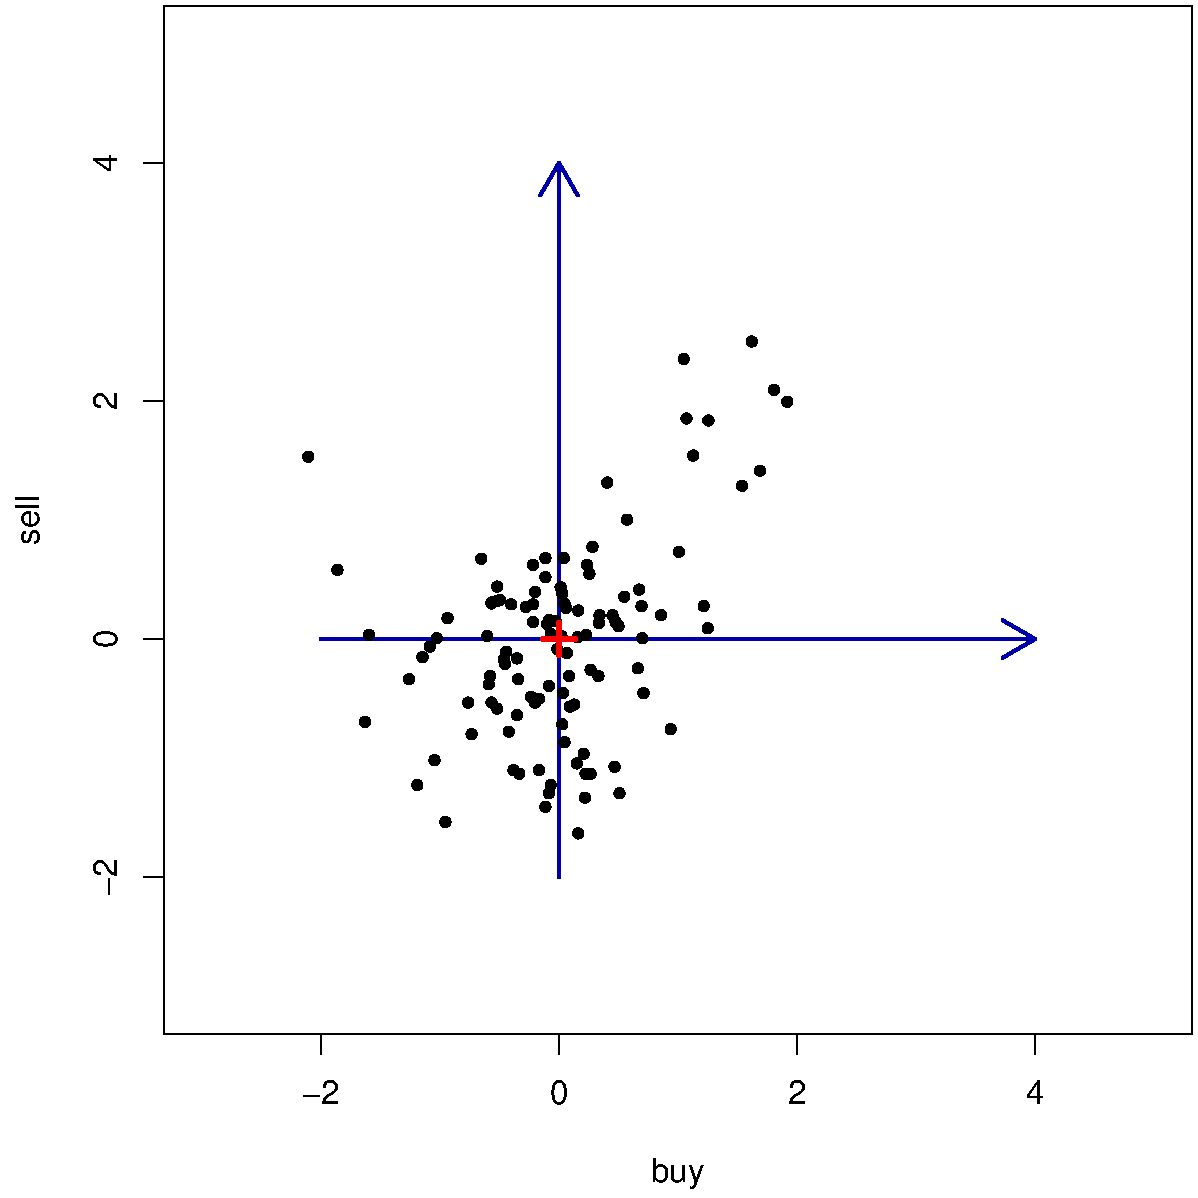
\includegraphics[width=6cm]{img/3_buy_sell_centered}}%
      \only<beamer:3| handout:3>{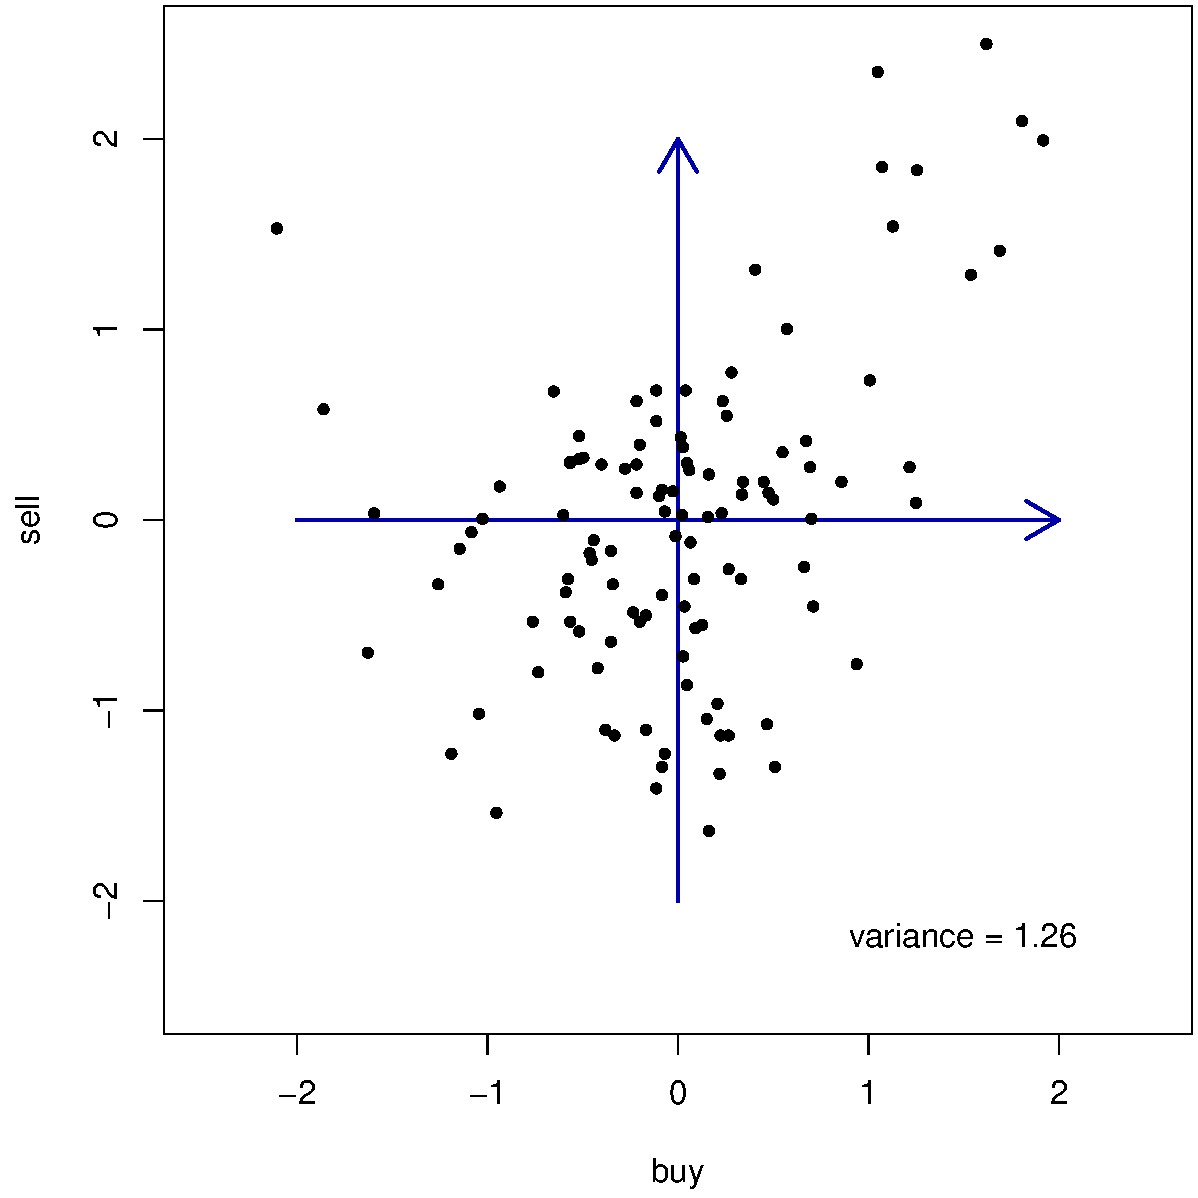
\includegraphics[width=6cm]{img/3_buy_sell_variance}}%
    \end{column}
  \end{columns}
\end{frame}

%%% Local Variables: 
%%% mode: latex
%%% TeX-master: "../../workspace"
%%% End: 


\begin{frame}
  \frametitle{Principal components analysis (PCA)}
  %% \framesubtitle{}

  \begin{itemize}
  \item We want to project the data points to a lower-dimensional subspace,
    but preserve distances as well as possible
  \item<2-> Insight 1: variance = average squared distance
    \[
    \frac{1}{k(k-1)} \sum_{i=1}^k \sum_{j=1}^k \norm{\vx[i] - \vx[j]}^2
    = \frac{2}{k-1} \sum_{i=1}^k \norm{\vx[i]}^2 = 2\sigma^2
    \]
  \item<3-> Insight 2: orthogonal projection always reduces distances\\
    \so difference in squared distances = loss of variance
  \item<4-> If we reduced the data set to just a single dimension,
    which dimension would still have the highest variance?
  \item<4-> Mathematically, we project the points onto a line through the origin
    and calculate one-dimensional variance on this line
    \begin{itemize}
    \item we'll see in a moment how to compute such projections
    \item but first, let us look at a few examples
    \end{itemize}
  \end{itemize}
\end{frame}

\begin{frame}<beamer:1-6| handout:1-3>[c]
  \frametitle{Projection and preserved variance: examples}
  %% \framesubtitle{}

  \begin{center}
    \only<beamer:1| handout:0>{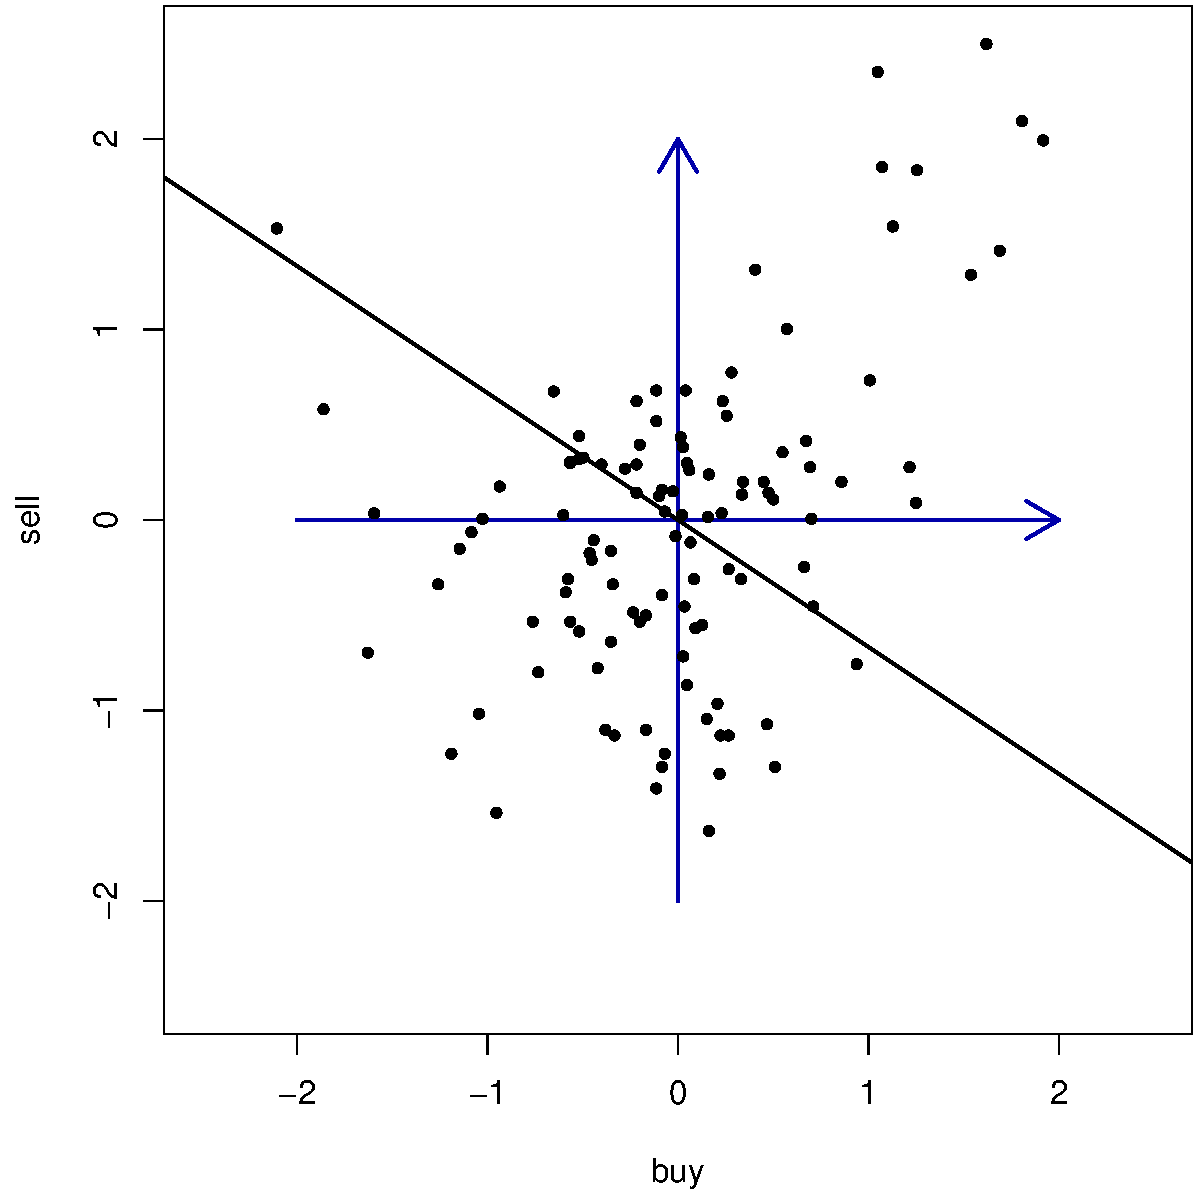
\includegraphics[width=7cm]{img/3_buy_sell_1_axis}}%
    \only<beamer:2| handout:1>{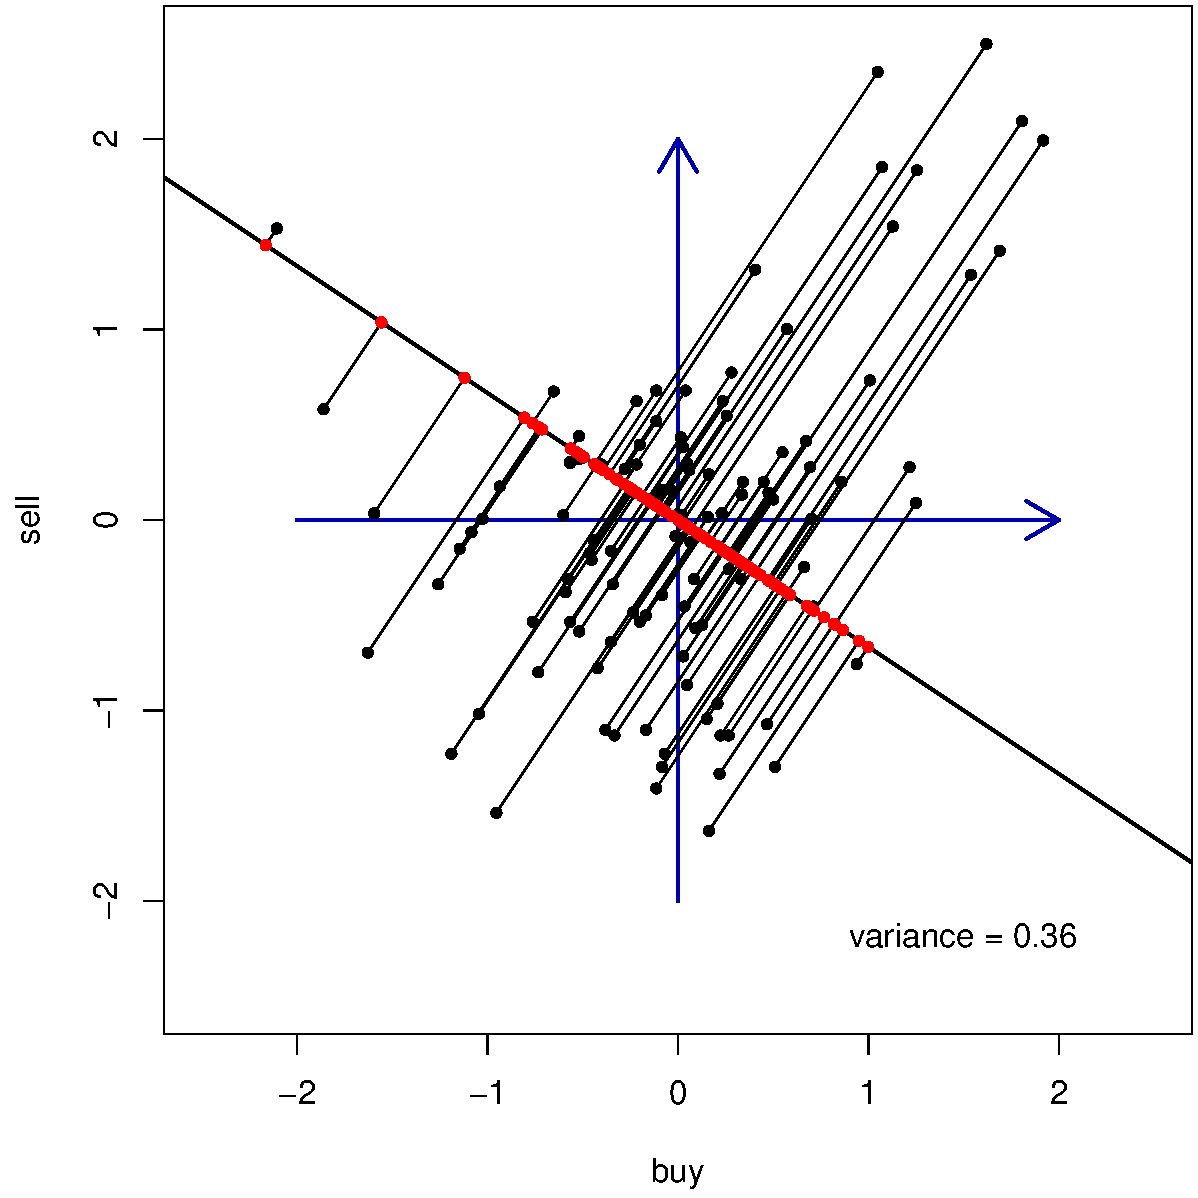
\includegraphics[width=7cm]{img/3_buy_sell_1_projection}}%
    \only<beamer:3| handout:0>{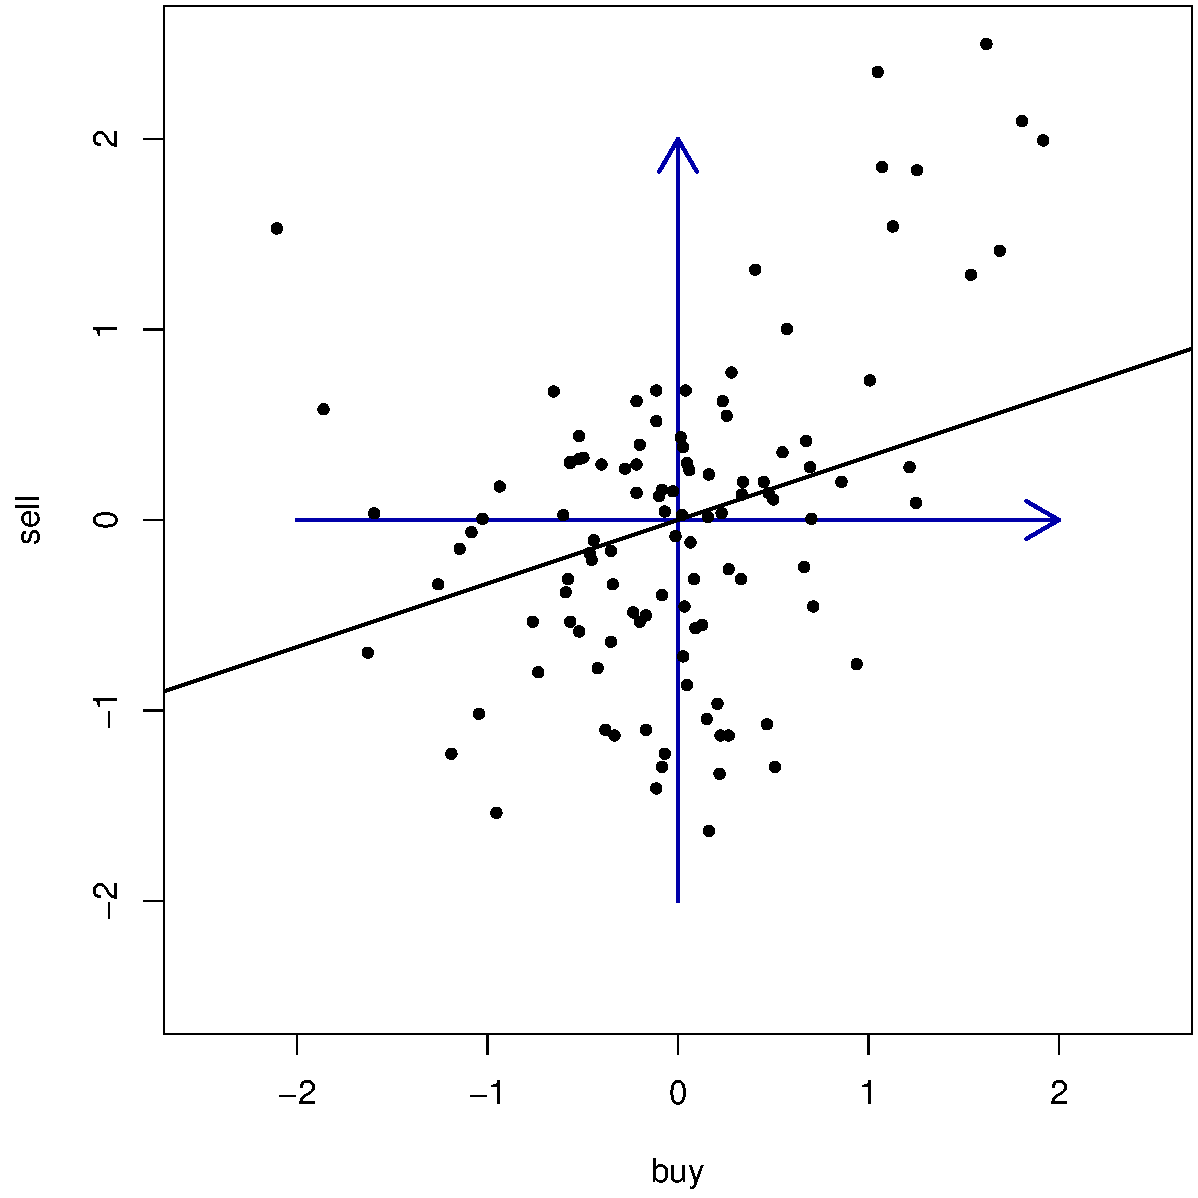
\includegraphics[width=7cm]{img/3_buy_sell_2_axis}}%
    \only<beamer:4| handout:2>{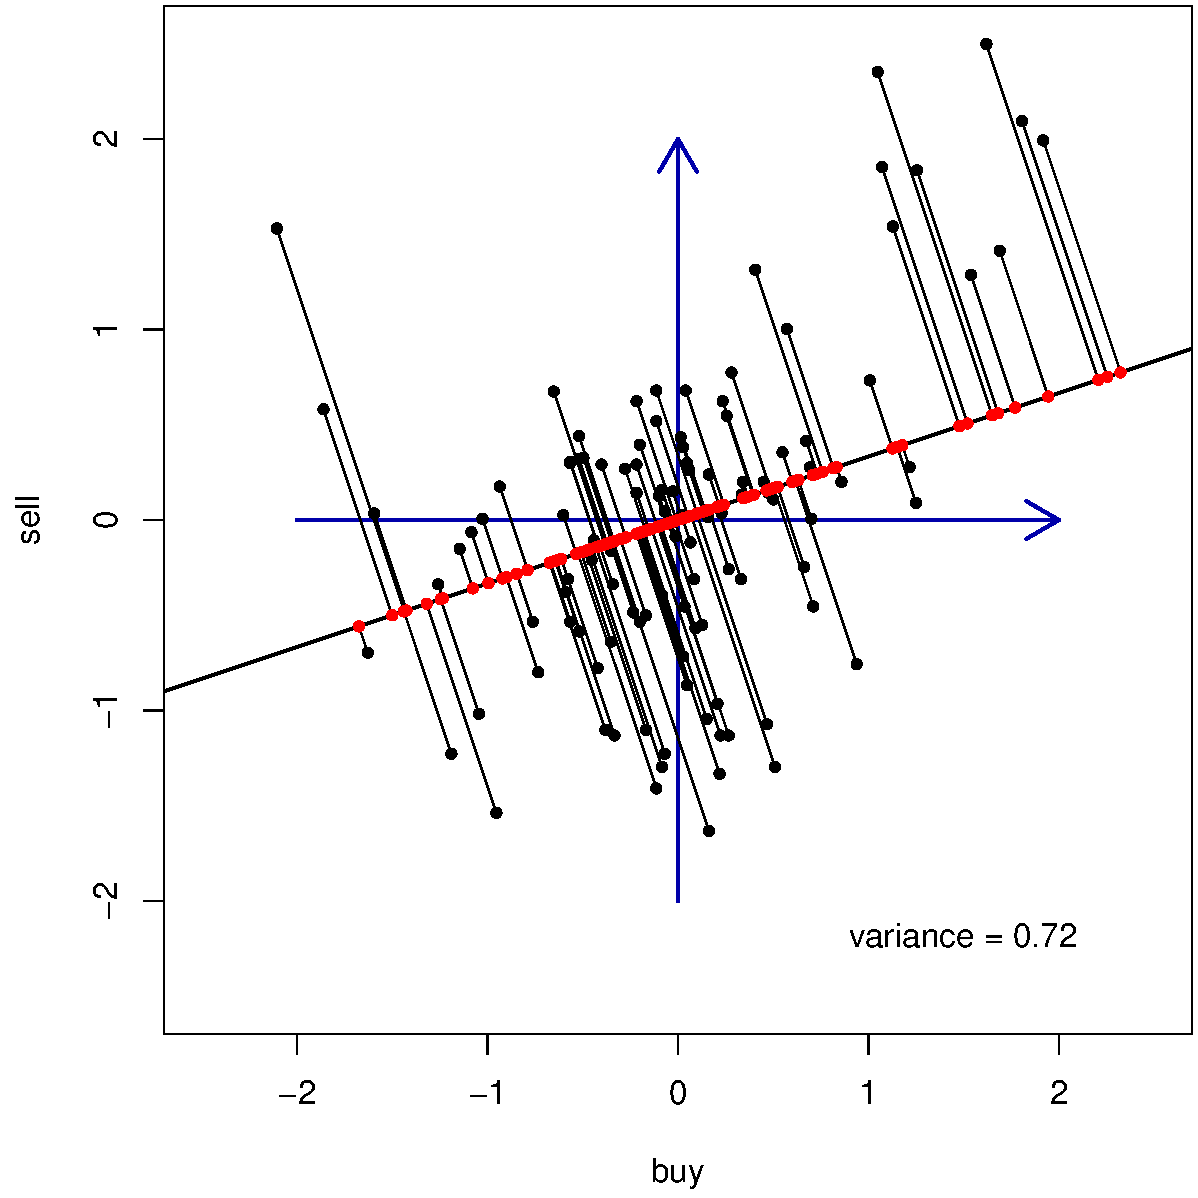
\includegraphics[width=7cm]{img/3_buy_sell_2_projection}}%
    \only<beamer:5| handout:0>{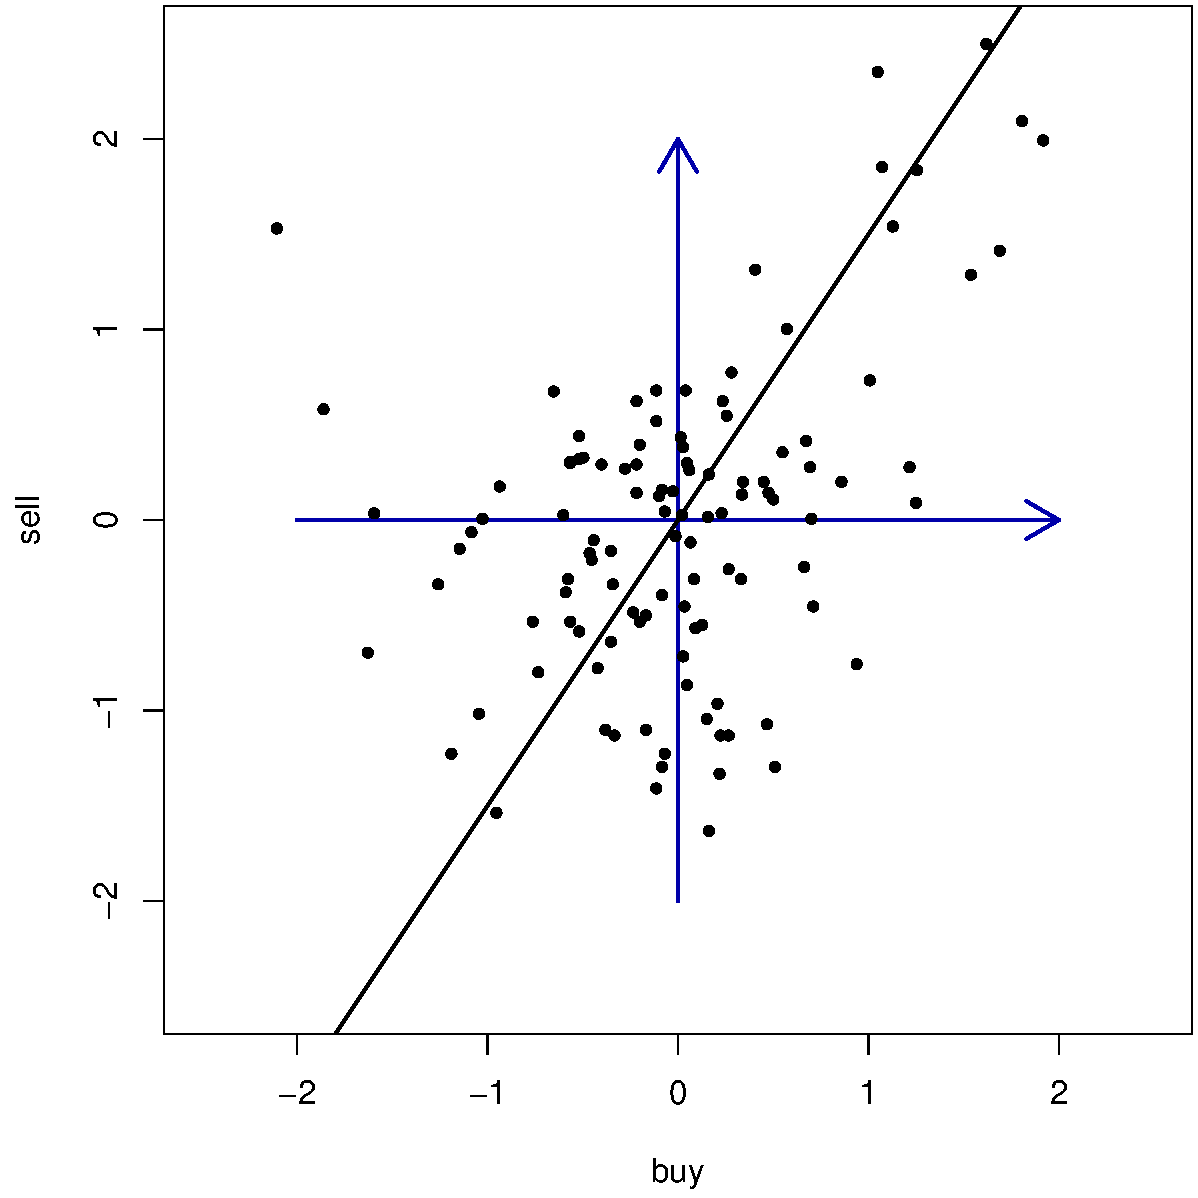
\includegraphics[width=7cm]{img/3_buy_sell_3_axis}}%
    \only<beamer:6| handout:3>{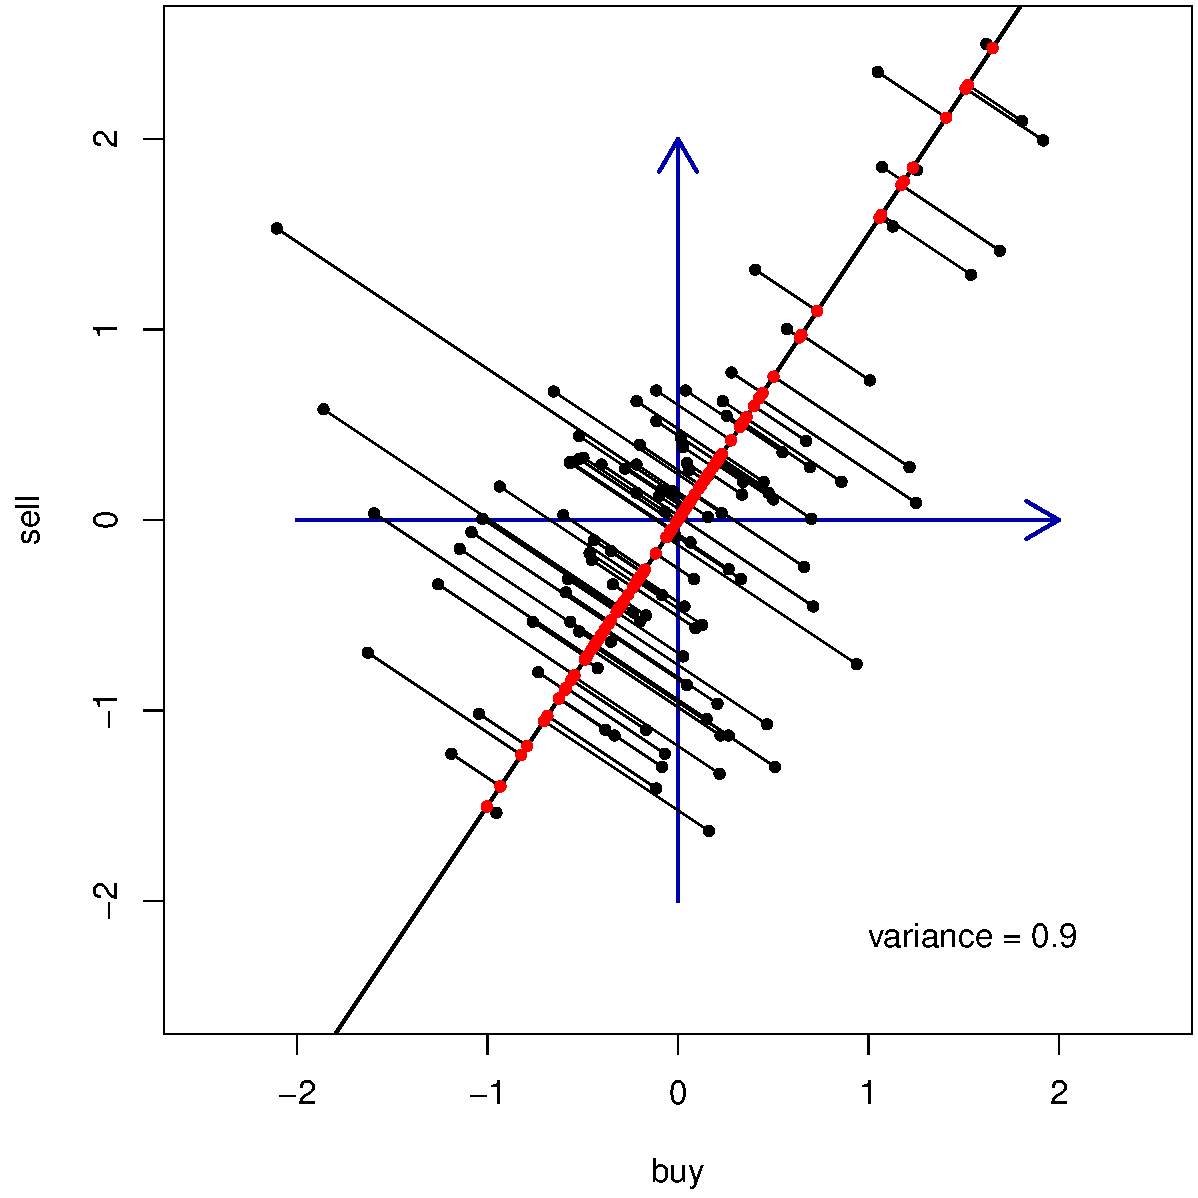
\includegraphics[width=7cm]{img/3_buy_sell_3_projection}}%
  \end{center}
\end{frame}

\begin{frame}
  \frametitle{The mathematics of projections}
  %% \framesubtitle{}

  \begin{columns}[c]
    \begin{column}{50mm}
      \begin{itemize}
      \item Line through origin given by unit vector
        $\norm{\vv} = 1$
      \item For a point $\vx$ and the corresponding unit vector $\vx' = \vx /
        \norm{\vx}$, we have \( \cos \varphi = \sprod{\vx'}{\vv} \)
      \end{itemize}
    \end{column}
    \begin{column}{50mm}
      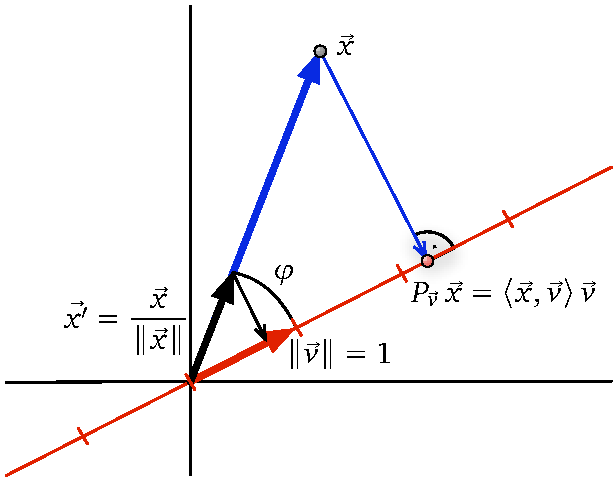
\includegraphics[width=50mm]{img/3_cosine_projection}
    \end{column}
  \end{columns}
  
  \pause
  \begin{itemize}
  \item Trigonometry: position of projected point on the line is
    $\norm{\vx}\cdot \cos\varphi = \norm{\vx}\cdot \sprod{\vx'}{\vv} =
    \sprod{\vx}{\vv}$
%  \item (projected point in original space is $\sprod{\vx}{\vv} \vv$)
  \item Preserved variance = one-dimensional variance on the line
    (note that data set is still centered after projection)
    \[
    \sigma_{\vv}^2 = \frac{1}{k-1} \sum_{i=1}^k \sprod{\vx_i}{\vv}^2
    \]
  \end{itemize}
\end{frame}

%%% Local Variables: 
%%% mode: latex
%%% TeX-master: "../../workspace"
%%% End: 


\begin{frame}
  \frametitle{The covariance matrix}
  %% \framesubtitle{}
  
  \begin{itemize}
  \item Find the direction $\vv$ with maximal $\sigma_{\vv}^2$, which is given by:
  \end{itemize}
  \ungap
  \begin{align*}
    \sigma_{\vv}^2 &= \tfrac{1}{k-1} \sum_{i=1}^k \sprod{\vx_i}{\vv}^2 
    \\
    \only<beamer:2-| handout:1>{
      &= \tfrac{1}{k-1} \sum_{i=1}^k \left(\vx_i^T \vv\right)^T
      \cdot \left(\vx_i^T \vv\right) }
    \\
    \only<beamer:3-| handout:1>{
      &= \tfrac{1}{k-1} \sum_{i=1}^k \vv^T  
      \left(\vx_i  \vx_i^T \right) \vv }
    \\
    \only<beamer:4-| handout:1>{
      &= \vv^T  
      \left( \tfrac{1}{k-1} \sum_{i=1}^k \vx_i \vx_i^T \right) 
      \vv} 
    \\
    \only<beamer:5-| handout:1>{
      &= \vv^T \mathbf{C} \vv}
  \end{align*}
\end{frame}

\begin{frame}
  \frametitle{The covariance matrix}
  %% \framesubtitle{}
  
  \begin{itemize}
  \item $\mathbf{C}$ is the \h{covariance matrix} of the data points
    \begin{itemize}
    \item $\mathbf{C}$ is a square $n\times n$ matrix ($2\times 2$ in our
      example)
    \end{itemize}
  \item Preserved variance after projection onto a line $\vv$ can easily be
    calculated as $\sigma_{\vv}^2 = \vv^T \mathbf{C} \vv$
  \item<2-> The original variance of the data set is given by $\sigma^2 =
    \mathop{\text{tr}}(\mathbf{C}) = C_{11} + C_{22} + \cdots + C_{nn}$
    \[
    \mathbf{C} =
    \begin{bmatrix}
      \primary{\sigma_1^2} & C_{12} & \cdots & C_{1n} \\
      C_{21} & \primary{\sigma_2^2} & \ddots & \vdots \\
      \\
      \vdots & \ddots & \primary{\ddots} & C_{n-1,n} \\
      \\
      C_{n1} & \cdots & C_{n,n-1}& \primary{\sigma_n^2}
    \end{bmatrix}
    \]
  \end{itemize}
\end{frame}

%%% Local Variables: 
%%% mode: latex
%%% TeX-master: "../../workspace"
%%% End: 


\begin{frame}
  \frametitle{Maximizing preserved variance}
  %% \framesubtitle{}

  \begin{itemize}
  \item In our example, we want to find the axis $\vv_1$ that preserves the
    largest amount of variance by maximizing $\vv_1^T \mathbf{C} \vv_1$
  \item<2-> For higher-dimensional data set, we also want to find the\\ axis
    $\vv_2$ with the second largest amount of variance, etc.
    \begin{itemize} 
    \item[\hand] Should not include variance that has already been accounted for:
      $\vv_2$ must be orthogonal to $\vv_1$, i.e.\ $\sprod{\vv_1}{\vv_2} = 0$
    \end{itemize}
  \item<3-> Orthogonal dimensions $\vv[1], \vv[2], \ldots$ \h{partition} variance:
    \[
    \sigma^2 = \sigma_{\vv[1]}^2 + \sigma_{\vv[2]}^2 + \ldots
    \]
  \item<4-> Useful result from linear algebra: every symmetric matrix
    $\mathbf{C} = \mathbf{C}^T$ has an \h{eigenvalue decomposition} with
    orthogonal \hh{eigenvectors} $\va_1, \va_2, \dots, \va_n$ and
    corresponding \hh{eigenvalues} $\lambda_1\geq \lambda_2\geq \dots \geq
    \lambda_n$
  \end{itemize}
\end{frame}

\begin{frame}
  \frametitle{Eigenvalue decomposition}
  %% \framesubtitle{}

  \begin{itemize}
  \item The eigenvalue decomposition of $\mathbf{C}$ can be written in the
    form
    \[
    \mathbf{C} = \mathbf{U}\cdot \mathbf{D}\cdot \mathbf{U}^T
    \]
    where $\mathbf{U}$ is an orthogonal matrix of eigenvectors (columns)
    and $\mathbf{D} = \mathop{\text{Diag}}(\lambda_1, \dots, \lambda_n)$ a diagonal
    matrix of eigenvalues
    \begin{small}
      \[
      \mathbf{U} =
      \begin{bmatrix}
        \vdots & \vdots & & \vdots \\
        \vdots & \vdots & & \vdots \\
        \va_1 & \va_2 & \cdots & \va_n \\
        \vdots & \vdots & & \vdots \\
        \vdots & \vdots & & \vdots
      \end{bmatrix}
      \qquad \mathbf{D} =
      \begin{bmatrix}
        \lambda_1 & & & \\
        & \lambda_2 & & & \\
        & & \ddots & & \\
        & & & \ddots & \\
        & & & & \lambda_n
      \end{bmatrix}
      \]
    \end{small}
    \begin{itemize}
    \item note that both $\mathbf{U}$ and $\mathbf{D}$ are $n\times n$ square matrices
    \end{itemize}
  \end{itemize}
\end{frame}

\begin{frame}
  \frametitle{The PCA algorithm}
  %% \framesubtitle{}

  \begin{itemize}
  \item With the eigenvalue decomposition of $\mathbf{C}$, we have 
    \[
    \sigma_{\vv}^2 = \vv^T \mathbf{C} \vv 
    = \vv^T \mathbf{U} \mathbf{D} \mathbf{U}^T \vv 
    = (\mathbf{U}^T \vv)^T \mathbf{D} (\mathbf{U}^T \vv) 
    = \vy^T \mathbf{D} \vy
    \]
    where $\vy = \mathbf{U}^T \vv$ = $[y_1, y_2, \ldots, y_n]^T$ are the
    coordinates of $\vv$ in the Cartesian basis formed by the eigenvectors of
    $\mathbf{C}$
  \item<2-> $\norm{\vy} = 1$ since $\mathbf{U}^T$ is an isometry (orthogonal matrix)
  \item<2-> We therefore want to maximize 
    \[
    \vv^T \mathbf{C} \vv = \lambda_1 (y_1)^2 + \lambda_2 (y_2)^2 \dots + \lambda_n (y_n)^2
    \]
    under the constraint $(y_1)^2 + (y_2)^2 + \dots + (y_n)^2 = 1$
  \item<3-> Solution: $\vy = [1, 0, \dots, 0]^T$ (since $\lambda_1$ is the
    largest eigenvalue)
  \item<3-> This corresponds to $\vv = \va_1$ (the first eigenvector of
    $\mathbf{C}$) and a preserved amount of variance given by $\sigma_{\vv}^2
    = \va_1^T \mathbf{C} \va_1 = \lambda_1$
  \end{itemize}
\end{frame}

\begin{frame}
  \frametitle{The PCA algorithm}
  %% \framesubtitle{}

  \begin{itemize}
  \item In order to find the dimension of second highest variance,\\
    we have to look for an axis $\vv$ orthogonal to $\va_1$
    \begin{itemize}
    \item[\hand] $\mathbf{U}^T$ is orthogonal, so the coordinates $\vy =
      \mathbf{U}^T \vv$ must be orthogonal to first axis $[1, 0, \dots, 0]^T$,
      i.e.\ $\vy = [0, y_2, \dots, y_n]^T$
    \end{itemize}
  \item<2-> In other words, we have to maximize
    \[
    \vv^T \mathbf{C} \vv = \lambda_2 (y_2)^2 \dots + \lambda_n (y_n)^2
    \]
    under constraints $y_1 = 0$ and $(y_2)^2 + \dots + (y_n)^2 = 1$
  \item<3-> Again, solution is $\vy = [0, 1, 0, \dots, 0]^T$, corresponding to the
    second eigenvector $\vv = \va_2$ and preserved variance $\sigma_{\vv}^2 =
    \lambda_2$
  \item<4-> Similarly for the third, fourth, \ldots\ axis
  \end{itemize}
\end{frame}

\begin{frame}
  \frametitle{The PCA algorithm}
  %% \framesubtitle{}

  \begin{itemize}
  \item The eigenvectors $\va_i$ of the covariance matrix $\mathbf{C}$ are
    called the \h{principal components} of the data set
  \item The amount of variance preserved (or ``explained'') by the $i$-th
    principal component is given by the eigenvalue $\lambda_i$
  \item Since $\lambda_1 \geq \lambda_2 \geq \dots \geq \lambda_n$, the first
    principal component accounts for the largest amount of variance etc.
  \item Coordinates of a point $\vx$ in PCA space are given by $\mathbf{U}^T
    \vx$ (note: these are the projections on the principal components)
  \item For the purpose of ``noise reduction'', only the first $n' < n$
    principal components (with highest variance) are retained, and the other
    dimensions in PCA space are dropped
    \begin{itemize}
    \item[\hand] i.e.\ data points are projected into the subspace $V$ spanned
      by the first $n'$ column vectors of $\mathbf{U}$
    \end{itemize}
  \end{itemize}
\end{frame}

\begin{frame}[c]
  \frametitle{PCA example}
  %% \framesubtitle{}

  \ungap
  \begin{center}
    \only<beamer:1| handout:0>{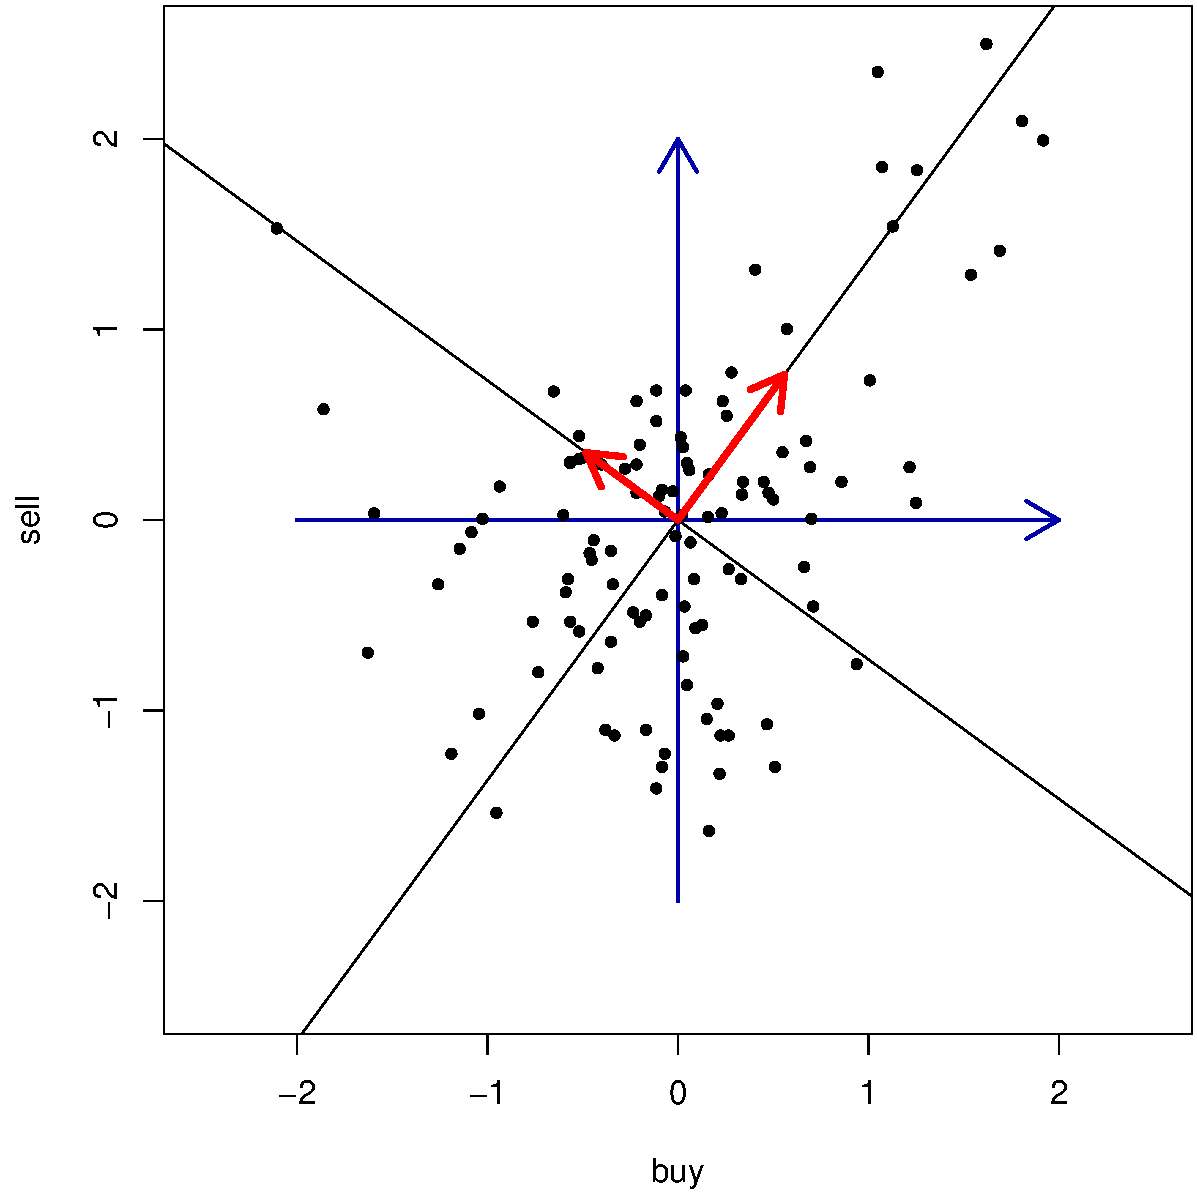
\includegraphics[width=8cm]{img/3_buy_sell_pca}}%
    \only<beamer:2| handout:1>{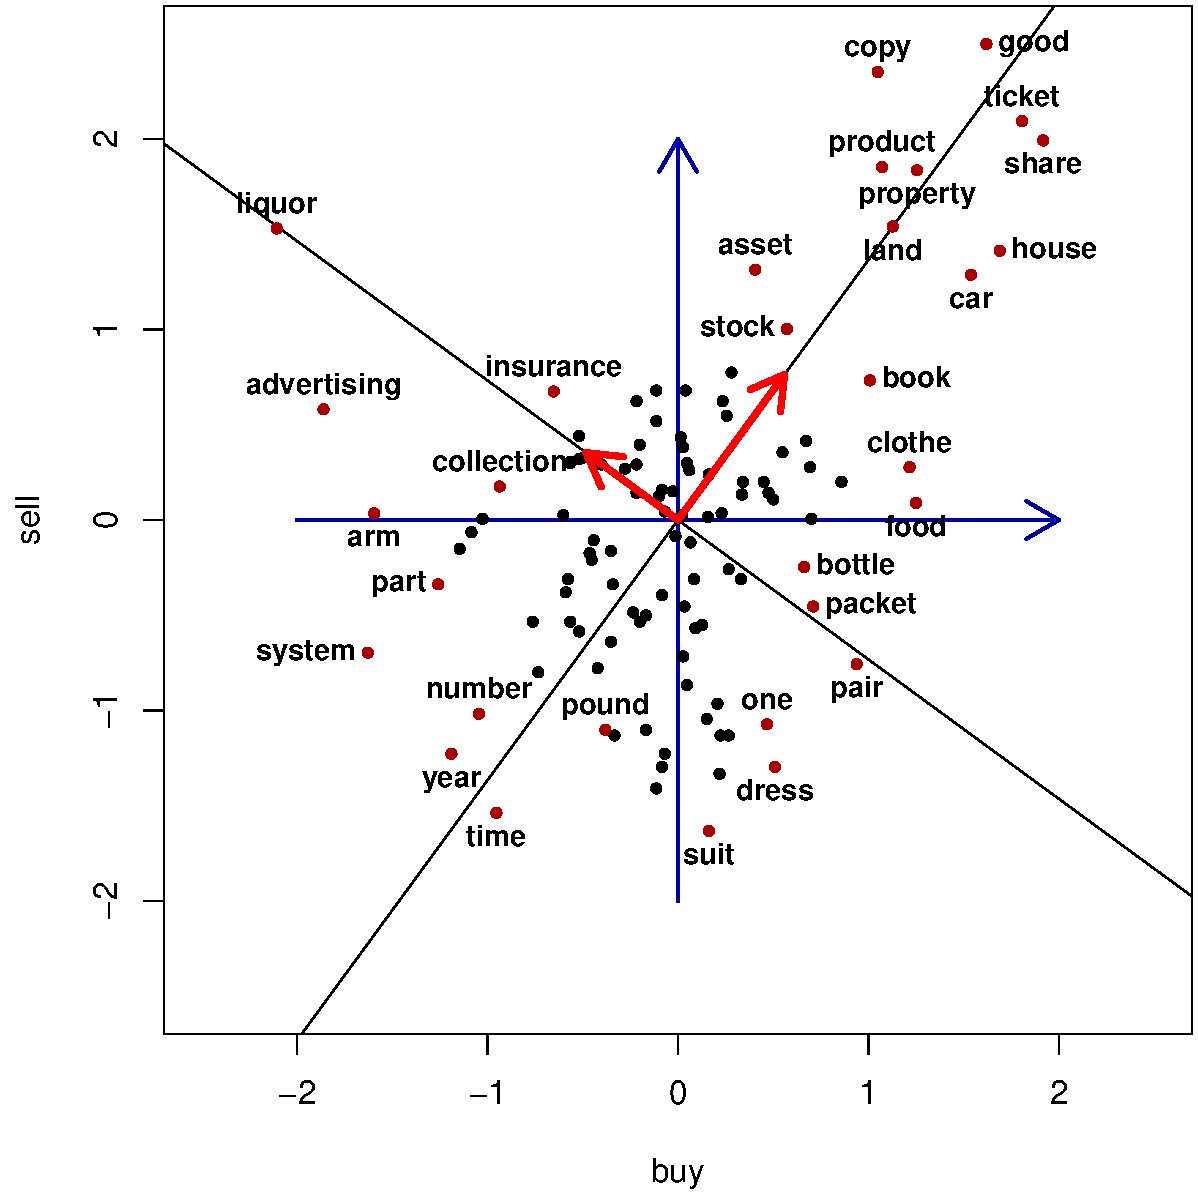
\includegraphics[width=8cm]{img/3_buy_sell_pca_labels}}%
  \end{center}
\end{frame}

%%% Local Variables: 
%%% mode: latex
%%% TeX-master: "../../workspace"
%%% End: 


% \begin{frame}[fragile]
  \frametitle{PCA in R}
  %% \framesubtitle{}
  
  \ungap
\begin{alltt}\small
> pca <- prcomp(M)  \REM{for the buy/sell example data}

> summary(pca) \begin{Rout}
Importance of components:
                         PC1   PC2
Standard deviation     0.947 0.599
Proportion of Variance 0.715 0.285
Cumulative Proportion  0.715 1.000 \end{Rout}

> print(pca) \begin{Rout}
Standard deviations:
[1] 0.9471326 0.5986067

Rotation:
            PC1        PC2
buy  -0.5907416  0.8068608
sell -0.8068608 -0.5907416 \end{Rout}
\end{alltt}
\end{frame}

\begin{frame}[fragile]
  \frametitle{PCA in R}
  %% \framesubtitle{}
  
  \ungap
\begin{alltt}\small
\REM{Coordinates in PCA space}
> pca\$x[c("house","book","arm","time"), ] \begin{Rout}
             PC1        PC2
house -2.1390957  0.5274687
book  -1.1864783  0.3797070
arm    0.9141092 -1.3080504
time   1.8036445  0.1387165 \end{Rout}

\REM{Transformation matrix \textbf{U}}
> pca\$rotation \begin{Rout}
            PC1        PC2
buy  -0.5907416  0.8068608
sell -0.8068608 -0.5907416 \end{Rout}

\REM{Eigenvalues of the covariance matrix \textbf{C}}
> (pca\$sdev)^2 \begin{Rout}
[1] 0.8970602 0.3583299 \end{Rout}
\end{alltt}
\end{frame}

%%% Local Variables: 
%%% mode: latex
%%% TeX-master: "../../workspace"
%%% End: 


%%%%%%%%%%%%%%%%%%%%%%%%%%%%%%%%%%%%%%%%%%%%%%%%%%%%%%%%%%%%%%%%%%%%%%
\subsection{SVD}

\begin{frame}
  \frametitle{Remember PCA?}
  %% \framesubtitle{}

  \begin{itemize}
  \item Principal components analysis is based on an \h{eigenvalue
      decomposition} of the \h{covariance matrix} $\mathbf{C}$ into
    \[
    \mathbf{C} = \mathbf{U}\cdot \mathbf{D}\cdot \mathbf{U}^T
    \]
    where $\mathbf{U}$ is orthogonal and $\mathbf{D} =
    \mathop{\text{Diag}}(\lambda_1, \ldots, \lambda_n)$.
  \item<2-> The columns of $\mathbf{U}$ are \hh{eigenvectors}
    \begin{center}
      $\mathbf{C} \va_i = \lambda_i \va_i$
    \end{center}
    for the ordered \hh{eigenvalues} $\lambda_1\geq \lambda_2\geq \dots \geq
    \lambda_n$
    \gap[.5]
  \item<3-> Interesting link: $\vu^T \mathbf{C} \vv$ describes a general
    \h{inner product}
    \begin{itemize}
    \item $\sigma_{\vv}$ is the norm of $\vv$ with respect to this general
      inner product
    \item the eigenvalue decomposition corresponds to a transformation into
      Cartesian coordinates where $\mathbf{C}$ has diagonal form
    \item eigenvalues $\lambda_i$ are the ``squashing factors'' of the unit
      circle
    \end{itemize}
  \end{itemize}
\end{frame}

\begin{frame}
  \frametitle{Singular value decomposition (SVD)}
  %% \framesubtitle{}

  \begin{itemize}
  \item The idea of eigenvalue decomposition can be generalised to an
    arbitrary (non-symmetric, non-square) matrix $\mathbf{A}$
    \begin{itemize}
    \item[\hand] need not have any eigenvalues
    \end{itemize}
  \item<2-> \h{Singular value decomposition} (\hh{SVD}) factorises $\mathbf{A}$ into
    \[
    \mathbf{A} = \mathbf{U}\cdot \Msigma\cdot \mathbf{V}^T
    \]
    where $\mathbf{U}$ and $\mathbf{V}$ are orthogonal coordinate
    transformations and $\Msigma$ is a rectangular-diagonal matrix of
    \hh{singular values}\\
    (with customary ordering $\sigma_1\geq \sigma_2\geq \dots \geq
    \sigma_n\geq 0$)
  \item<3-> SVD is an important tool in linear algebra and statistics
    \begin{itemize}
    \item[\hand] in particular, PCA can be computed from SVD decomposition
    \end{itemize}
  \end{itemize}
\end{frame}

\begin{frame}[c]
  \frametitle{SVD illustration}
  %% \framesubtitle{}
  
  \begin{equation*}
    \begin{bmatrix}
      & & \primary{n} & & \\
      & & & & \\
      & & & & \\
      \primary{k} & & \mathbf{A} & & \\
      & & & & \\
      & & & & \\
      & & & & 
    \end{bmatrix}
    =
    \begin{bmatrix}
      & & & \primary{k} & & & \\
      & & & & & & \\
      & & & & & & \\
      \primary{k} & & & \mathbf{U} & & & \\
      & & & & & & \\
      & & & & & & \\
      & & & & & &
    \end{bmatrix}
    \cdot
    \begin{bmatrix}
      \sigma_1 & \primary{n} & \\
      & \ddots & \\
      & & \sigma_n \\
      \primary{k} & \Msigma & \\
      & & \\
      & & \rule{0mm}{5mm} 
    \end{bmatrix}
    \cdot
    \begin{bmatrix}
      & & \primary{n} & & \\
      & & & & \\
      \primary{n} & & \mathbf{V}^T & & \\
      & & & & \\
      & & & &
    \end{bmatrix}
  \end{equation*}
\end{frame}

%%% Local Variables: 
%%% mode: latex
%%% TeX-master: "../../workspace"
%%% End: 


\begin{frame}
  \frametitle{PCA and the DSM matrix}
  %% \framesubtitle{}
  \begin{itemize}
  \item Take a closer look at the covariance matrix
    \[
    \mathbf{C} = \tfrac{1}{k-1} \sum_{i=1}^k \vx_i \vx_i^T
    \]
  \item<2-> With $\vx_i^T = \bigl[ x_{i1}, \ldots, x_{in} \bigr]$ we find that
    \[
    \vx_i \vx_i^T
    =
    \begin{bmatrix}
      x_{i1} \\ \vdots \\ x_{in}
    \end{bmatrix}
    \cdot
    \begin{bmatrix}
      x_{i1} & \cdots & x_{in}
    \end{bmatrix}    
    =
    \begin{bmatrix}
      (x_{i1})^2 & x_{i1} x_{i2} & \cdots & x_{i1} x_{in} \\
      x_{i2} x_{i1} & (x_{i2})^2 & \cdots &  x_{i2} x_{in} \\
      \vdots & \vdots & \ddots & \vdots \\
      x_{in} x_{i1} & x_{in} x_{i2} & \cdots & (x_{in})^2
    \end{bmatrix}
    \]
  \end{itemize}
\end{frame}

\begin{frame}
  \frametitle{PCA and the DSM matrix}
  %% \framesubtitle{}
  \[
  \sum_{i=1}^k \vx_i \vx_i^T
  =
  \begin{bmatrix}
    \sum_i (x_{i1})^2 & \sum_i x_{i1} x_{i2} & \cdots & \sum_i x_{i1} x_{in} \\
    \sum_i x_{i2} x_{i1} & \sum_i (x_{i2})^2 & \cdots & \sum_i x_{i2} x_{in} \\
    \vdots & \vdots & \ddots & \vdots \\
    \sum_i x_{in} x_{i1} & \sum_i x_{in} x_{i2} & \cdots & \sum_i (x_{in})^2
  \end{bmatrix}
  \]
  \begin{itemize}
  \item<2-> If the $\vx_i$ are the \primary{row} vectors of a DSM matrix
    $\mathbf{M}$, then the sums above are inner products between its
    \primary{column} vectors 
  \item<3->[\So] $\mathbf{C}$ can efficiently be computed by matrix multiplication
    (similar to cosine similarities, but for column vectors)
    \[
    \mathbf{C} = \tfrac{1}{k-1} \sum_{i=1}^k \vx_i \vx_i^T
    = \tfrac{1}{k-1} \mathbf{M}^T \mathbf{M}
    \]
  \end{itemize}
\end{frame}

\begin{frame}
  \frametitle{PCA by singular value decomposition}
  %% \framesubtitle{}
  \begin{itemize}
  \item Up to an irrelevant scaling factor $\tfrac{1}{k-1}$, we are thus
    looking for an eigenvalue decomposition of $\mathbf{M}^T \mathbf{M}$
    (which is symmetric!)
  \item Like every matrix, $\mathbf{M}$ has a singular value decomposition
    \[
    \mathbf{M} = \mathbf{U} \Msigma \mathbf{V}^T
    \]
  \item By inserting the SVD, we obtain
    \begin{align*}
      \mathbf{M}^T \mathbf{M}
      &= \bigl(\mathbf{U} \Msigma \mathbf{V}^T\bigr)^T
      \mathbf{U} \Msigma \mathbf{V}^T
      \\
      &= (\mathbf{V}^T)^T \Msigma^T 
      \underbrace{ \mathbf{U}^T \mathbf{U} }_{\mathbf{I}}
      \Msigma \mathbf{V}^T
      \\
      &= \mathbf{V} \bigl( 
      \underbrace{ \Msigma^T \Msigma }_{\mathbf{\Msigma^2}}
      \bigr) \mathbf{V}^T
    \end{align*}
  \end{itemize}
\end{frame}

\begin{frame}
  \frametitle{PCA by singular value decomposition}
  %% \framesubtitle{}
  \begin{itemize}
  \item We have found the eigenvalue decomposition
    \[
    \mathbf{M}^T \mathbf{M} = \mathbf{V} \Msigma^2 \mathbf{V}^T
    \]
    with
    \[
    \Msigma^2 = \Msigma^T \Msigma
    =
    \begin{bmatrix}
      (\sigma_1)^2 & \primary{n} & \rule{0mm}{5mm} \\
      \primary{n} & \ddots & \rule{0mm}{5mm} \\
      \rule{0mm}{6mm} & & (\sigma_n)^2 
    \end{bmatrix}
    \]
  \item<2-> The column vectors of $\mathbf{V}$ are \h{latent dimensions}
  \item<3-> The corresponding squared \h{singular values} partition variance:
    $(\sigma_1)^2 / \sum_i (\sigma_i)^2$ = proportion along first latent
    dimension
    \begin{itemize}
    \item[\hand] intuitively, singular value shows importance of latent dimension
    \end{itemize}
  \item<4-> Interpretation of $\mathbf{U}$ is less intuitive (\h{latent families}
    of words?)
  \end{itemize}
\end{frame}

\begin{frame}
  \frametitle{Transforming the DSM matrix}
  %% \framesubtitle{}

  \begin{itemize}
  \item We can directly transform the columns of the DSM matrix $\mathbf{M}$:
    \[
    \mathbf{M} \mathbf{V} 
    = \mathbf{U} \Msigma (\mathbf{V}^T \mathbf{V})
    = \mathbf{U} \Msigma
    \]
    \pause\ungap[1.5]
  \item For ``noise reduction'', project into $m$-dimensional subspace\\
    by dropping all but the first $m \ll n$ columns of $\mathbf{U} \Msigma$
  \item[\So] Sufficient to calculate the first $m$ \h{singular values}
    $\sigma_1,\ldots, \sigma_m$ and \h{left singular vectors} $\va_1,\ldots,
    \va_m$ (columns of $\mathbf{U}$)
  \item[]\pause
  \item What is the difference between SVD and PCA?%
    \pause
    \begin{itemize}
    \item[\hand] we forgot to center and rescale the data!
    \item[\hand] most DSM matrices contain only non-negative values
    \item[\hand] first latent dimension points towards ``positive'' sector,
      and was often found to be ``uninteresting'' in early SVD studies
    \end{itemize}
  \end{itemize}
\end{frame}

%%% Local Variables: 
%%% mode: latex
%%% TeX-master: "../../workspace"
%%% End: 


% \subsection{with R}
%\begin{frame}[fragile]
  \frametitle{SVD with R}
  %% \framesubtitle{}

\ungap
\begin{alltt}\small 
\REM{As an example, we will use the unscaled matrix \textbf{M} again}
> M1 <- M[c(1, 2, 4, 6), ]
> M1 \begin{Rout}       
        eat get hear kill see use
  boat    0  59    4    0  39  23
  cat     6  52    4   26  58   4
  dog    33 115   42   17  83  10
  pig     9  12    2   27  17   3 \end{Rout}

\REM{\texttt{svd()} function returns data structure with decomposition}
> SVD <- svd(M1)

> SVD\$d  \REM{singular values} \begin{Rout}
[1] 186.57942  34.92487  28.18571  12.03908  \end{Rout}
\end{alltt}
\end{frame}

\begin{frame}[fragile]
  \frametitle{SVD with R}
  %% \framesubtitle{}

\ungap
\begin{alltt}\small
\REM{Extract matrices \textbf{U}, \(\Msigma\) and \textbf{V}}
> Sigma <- diag(SVD\$d)  \REM{reduced to square matrix}
> U <- SVD\$u  \REM{coordinate transformations \textbf{U} and \textbf{V}}
> V <- SVD\$v  \REM{recall that \textbf{V} contains the latent dimensions}

\REM{Now reconstruct \textbf{M} from decomposition }
> round(U \%*\% Sigma \%*\% t(V), 2) \begin{Rout}
     [,1] [,2] [,3] [,4] [,5] [,6]
[1,]    0   59    4    0   39   23
[2,]    6   52    4   26   58    4
[3,]   33  115   42   17   83   10
[4,]    9   12    2   27   17    3 \end{Rout}

\end{alltt}
\end{frame}


\begin{frame}[fragile]
  \frametitle{SVD with R}
  %% \framesubtitle{}

\ungap
\begin{alltt}\small
\REM{Coordinates of target nouns in latent DSM space}
> U \%*\% Sigma

> M1 \%*\% V  \REM{this version preserves row names}
             [,1]       [,2]       [,3]       [,4]
  boat  -69.97214 -12.570114  21.760062  4.4036025
  cat   -78.87562  21.092424   9.865719 -6.9580067
  dog  -151.85390  -9.004136 -14.673158  0.1279540
  pig   -25.19541  23.146798  -2.880942  8.7816522
\end{alltt}
\end{frame}


\begin{frame}[fragile]
  \frametitle{SVD with R}
  %% \framesubtitle{}

\ungap
\begin{alltt}\small 
\REM{Compute rank-\(m\) approximations of the original matrix \textbf{M}}
> svd.approx <- function (m) \{
+   U[,1:m, drop=FALSE] \%*\% Sigma[1:m,1:m, drop=FALSE] \%*\% 
+   t(V)[1:m,, drop=FALSE]
+ \}
> round(svd.approx(1), 1) \begin{Rout}
     [,1]  [,2] [,3] [,4] [,5] [,6]
[1,] 11.5  52.3 14.1 10.7 40.9  7.1
[2,] 12.9  58.9 15.9 12.0 46.1  8.0
[3,] 24.9 113.4 30.6 23.2 88.7 15.4
[4,]  4.1  18.8  5.1  3.8 14.7  2.5 \end{Rout}
> round(svd.approx(2), 1) \begin{Rout}
     [,1]  [,2] [,3] [,4] [,5] [,6]
[1,] 11.1  56.4 17.2  0.2 37.0  9.4
[2,] 13.6  51.9 10.8 29.7 52.6  4.1
[3,] 24.6 116.4 32.8 15.6 85.9 17.0
[4,]  4.8  11.2 -0.6 23.2 21.9 -1.7 \end{Rout}
\end{alltt}
\end{frame}

%%% Local Variables: 
%%% mode: latex
%%% TeX-master: "../../workspace"
%%% End: 


%%%%%%%%%%%%%%%%%%%%%%%%%%%%%%%%%%%%%%%%%%%%%%%%%%%%%%%%%%%%%%%%%%%%%%
\subsection{High-dimensional DSM}

\begin{frame}
  \frametitle{Scaling up to the real world}
  %% \framesubtitle{}

  \begin{itemize}
  \item So far, we have worked on small \hh{toy models}
    \begin{itemize}
    \item DSM matrix restricted to 2,000 -- 5,000 rows and columns
    \item small corpora (or dependency sets) can be processed within
      \textbf{R}
    \end{itemize}
    \pause
  \item Now we need to scale up to \h{real world} data sets
    \begin{itemize}
    \item for most statistical models, more data are better data!
    \item cf.\ success of Google-based NLP techniques (even if simplistic)
    \end{itemize}
    \pause
  \item Example 1: window-based DSM on BNC content words
    \begin{itemize}
    \item 83,926 lemma types with $f\geq 10$
    \item term-term matrix with 83,926 $\cdot$ 83,926 = 7 billion entries
    \item standard representation requires 56 GB of RAM (8-byte floats)%
      \pause
    \item only 22.1 million non-zero entries ($= 0.32\%$)
    \end{itemize}
    \pause
  \item Example 2: Google Web 1T 5-grams (1 trillion words)
    \begin{itemize}
    \item more than 1 million word types with $f\geq 2500$
    \item term-term matrix with 1 trillion entries requires 8 TB RAM
    \item only 400 million non-zero entries ($= 0.04\%$)
    \end{itemize}
  \end{itemize}
\end{frame}

\begin{frame}
  \frametitle{Handling large data sets: three approaches}
  %% \framesubtitle{}

  \begin{enumerate}
  \item Sparse matrix representation
    \begin{itemize}
    \item full DSM matrix does not fit into memory
    \item but much smaller number of non-zero entries can be handled
    \item[] \pause
    \end{itemize}
  \item Feature selection
    \begin{itemize}
    \item reduce DSM matrix to subset of columns (usu.\ 2,000 -- 10,000)
    \item select most frequent, salient, discriminative, \ldots\ features
    \item[] \pause
    \end{itemize}
  \item Dimensionality reduction
    \begin{itemize}
    \item also reduces number of columns, but maps vectors to subspace
    \item singular value decomposition (usu.\ ca.\ 300 dimensions)
    \item random indexing (2,000 or more dimensions)
    \item performed with external tools \so \textbf{R} can handle reduced matrix
    \end{itemize}
  \end{enumerate}
\end{frame}

%%% Local Variables: 
%%% mode: latex
%%% TeX-master: "../../workspace"
%%% End: 


\begin{frame}
  \frametitle{Sparse matrix representation}
  %% \framesubtitle{}

  \ungap
  \begin{itemize}
  \item Invented example of a \hh{sparsely populated} DSM matrix
    \begin{center}\footnotesize
      \begin{tabular}{r | cccccc}
        & eat & get & hear & kill & see & use \\
        \midrule
        boat  &   $\cdot$  & 59  &   $\cdot$  &   $\cdot$  & 39 &  23 \\
        cat   &   $\cdot$  &  $\cdot$  &   $\cdot$  &  26  & 58 &   $\cdot$ \\
        cup   &   $\cdot$  & 98  &   $\cdot$  &   $\cdot$  &  $\cdot$ &   $\cdot$ \\
        dog   &  33  &  $\cdot$  &  42  &   $\cdot$  & 83 &   $\cdot$ \\
        knife &   $\cdot$  &  $\cdot$  &   $\cdot$  &   $\cdot$  &  $\cdot$ &  84 \\
        pig   &   9  &  $\cdot$  &   $\cdot$  &  27  &  $\cdot$ &   $\cdot$ 
      \end{tabular}
    \end{center}
    \gap\pause
  \item Store only non-zero entries in compact \h{sparse matrix format}
    \begin{center}\footnotesize
      \begin{tabular}{r|r|r c r|r|r}
        row & col & value && row & col & value \\
        \cline{1-3} \cline{5-7}
        1  &  2  &  59 &&  4  &  1  &  33 \\
        1  &  5  &  39 &&  4  &  3  &  42 \\
        1  &  6  &  23 &&  4  &  5  &  83 \\
        2  &  4  &  26 &&  5  &  6  &  84 \\
        2  &  5  &  58 &&  6  &  1  &   9 \\
        3  &  2  &  98 &&  6  &  4  &  27 \\
       \end{tabular}
    \end{center}
  \end{itemize}
\end{frame}

\begin{frame}
  \frametitle{Working with sparse matrices}
  %% \framesubtitle{}

  \begin{itemize}
  \item Compressed format: each row index (or column index) stored only once,
    followed by non-zero entries in this row (or column)%
    \begin{itemize}
    \item convention: \h{column-major} matrix (data stored by columns)
    \item[]
    \end{itemize}
    \pause
  \item Specialised algorithms for sparse matrix algebra
    \begin{itemize}
    \item especially matrix multiplication, solving linear systems, etc.
    \item take care to avoid operations that create a dense matrix!
    \item[]
    \end{itemize}
    \pause
  \item \textbf{R} implementation: \texttt{Matrix} package (from CRAN)
    \begin{itemize}
    \item can build sparse matrix from (row, column, value) table
    \item unfortunately, no implementation of sparse SVD so far
    \item[]
    \end{itemize}
    \pause
  \item Other software packages: Matlab, Octave (recent versions)
  \end{itemize}
\end{frame}

%%% Local Variables: 
%%% mode: latex
%%% TeX-master: "../../workspace"
%%% End: 


\begin{frame}
  \frametitle{Feature selection}
  %% \framesubtitle{}

  \begin{itemize}
  \item Many published models use \h{feature selection} to reduce\\
    the size of a term-term DSM matrix%
    \pause
  \item Selection criteria:
    \begin{itemize}
    \item most frequent context terms
    \item most informative contxt terms (tf.idf)
    \item most discriminative context terms (variance, entropy)
    \item term restricted by part of speech (e.g.\ only verbs)
    \end{itemize}
    \pause
  \item Features often selected \emph{before} co-occurrence counts
    \begin{itemize}
    \item only a moderately-sized DSM matrix has to be built
    \item allows simple in-memory algorithm for co-occurrence counts
    \end{itemize}
    \pause
  \item Alternative: build DSM matrix only for relevant target terms
    \begin{itemize}
    \item i.e.\ reduce the number of rows instead of number of columns
    \end{itemize}
    \pause
  \item \hh{Disadvantage}: useful information may be discarded
    \begin{itemize}
    \item aggressive feature selection is common in the DSM literature
    \end{itemize}
  \end{itemize}
\end{frame}

%%% Local Variables: 
%%% mode: latex
%%% TeX-master: "../../workspace"
%%% End: 


\begin{frame}
  \frametitle{Dimensionality reduction: SVD}
  %% \framesubtitle{}

  \begin{itemize}
  \item Feature selection is a simple form of \h{dimensionality reduction} for
    managing high-dimensional spaces
    \begin{itemize}
    \item information from discarded features is completely lost
    \end{itemize}
    \pause
  \item Better strategy: only discard irrelevant information by orthogonal
    projection into subspace of latent dimensions
    \begin{itemize}
    \item subspace of first $m$ principal components or singular vectors
    \item recall that this subspace preserves original distances as well as
      possible \so minimal amount of information discarded
    \end{itemize}
    \pause
  \item Key ingredient: implementation of \h{sparse-matrix SVD}
    \begin{itemize}
    \item SVDPACK with various algorithms developed by Michael Berry
    \item most convenient implementation: SVDLIBC\\
      \url{http://tedlab.mit.edu/~dr/svdlibc/}
    \item standard input format: compressed column-major sparse matrix
    \item only calculates first $m$ singular values and vectors
    \end{itemize}
    \pause
  \item SVD components $\mathbf{U}$, $\Msigma$ and $\mathbf{V}$ are stored in
    separate files
  \end{itemize}
\end{frame}

\begin{frame}
  \frametitle{Dimensionality reduction: Random Indexing}
  %% \framesubtitle{}

  \begin{itemize}
  \item SVD is computationally expensive for large DSM matrix
    \begin{itemize}
    \item even if the matrix is sparsely populated
    \end{itemize}
    \pause
  \item Cheap method: orthogonal projection into \hh{random} subspace
    \begin{itemize}
    \item it can be shown that this preserves original distances with high
      probability (though not as well as SVD)
    \item intuition: if dimensionality $m$ of subspace is large enough, some
      vector should be close to $\va_1$, another close to $\va_2$, etc.
    \end{itemize}
    \So \h{random indexing} (\hh{RI})%
    \pause
  \item Further simplication: use \hh{random basis} vectors for subspace
    \begin{itemize}
    \item saves additional cost of constructing an orthonormal basis
    \item if dimensionality $n$ of original DSM space is large enough,\\
      two random vectors are likely to be almost orthogonal
    \item intuition: inner product between random vectors = covariance of two
      independent samples of random numbers (should be 0)
    \end{itemize}
    \pause
  \item SVD identifies latent dimensions (``noise reduction''), but RI only
    preserves distances \so requires higher dimensionality $m$
  \end{itemize}
\end{frame}

%%% Local Variables: 
%%% mode: latex
%%% TeX-master: "../../workspace"
%%% End: 




%%% Local Variables: 
%%% mode: latex
%%% TeX-master: "../workspace"
%%% End: 



%%%%%%%%%%%%%%%%%%%%%%%%%%%%%%%%%%%%%%%%%%%%%%%%%%%%%%%%%%%%%%%%%%%%%%
%% References (if any)

% \frame[allowframebreaks]{
%   \frametitle{References}
%   \bibliographystyle{natbib-stefan}
%   \begin{scriptsize}
%     \bibliography{dsm,stefan-literature,stefan-publications}
%   \end{scriptsize}
% }

\end{document}
